\documentclass[12pt,a4paper,listof=totoc]{scrartcl}
\usepackage{fontspec}
\setmainfont{Times New Roman}
\setromanfont{Times New Roman}
\addtokomafont{disposition}{\normalfont\bfseries}
\usepackage{microtype} % fix overfull hboxes nicely
\usepackage[onehalfspacing]{setspace}
\usepackage[
    breaklinks=true,
    colorlinks=false,
    pdfborder={0 0 0},
    pdfauthor={Benedikt Schnur},
    pdftitle={Bachelor Thesis},
    unicode=true
]{hyperref}
\usepackage{titling}
\usepackage{ragged2e}
\usepackage{tikz}
\usepackage{xcolor}					% Farben
\newcommand*{\email}[1]{            % Klickbare eMail-Adressen
    \normalsize\href{mailto:#1}{#1}\par
    }
\usepackage{booktabs}				% "Schöne" Tabellen
\usepackage{csquotes}               % Empfohlener Import für babel/polyglossia
\usepackage{float}                  % Bessere Platzierungsmöglichkeiten von floats
\usepackage{siunitx}                % Einheitliche Darstellung von Werten mit ihren Einheiten
\sisetup{
    detect-all,
    per-mode = symbol,
    range-phrase = --
}

\usepackage{amsmath}
\usepackage{amssymb}

\usepackage{acro}
\acsetup{make-links=true}

\usepackage[section]{placeins}      % Bilder bleiben im Abschnitt
\let\Oldsubsection\subsection
\renewcommand{\subsection}{\FloatBarrier\Oldsubsection}

\usepackage[left=2cm,right=2cm,top=2cm,bottom=2cm,headheight=18pt,headsep=1.365cm,footskip=1cm,footnotesep=1.365cm]{geometry}
\usepackage{scrlayer-scrpage}
%\setlength{\headheight}{2cm}
%\setlength{\footheight}{2cm}
\RedeclareSectionCommands[
  beforeskip=12pt,
  afterskip=6pt]{section,subsection,subsubsection,paragraph,subparagraph}
\setlength{\parskip}{6pt}
\setlength{\parindent}{0em} 

\usepackage[
    backend=biber,
    style=ieee,
    maxcitenames=2,	% mindestens 2 Namen ausgeben bevor et. al. kommt
    mincitenames=1,
    maxbibnames=6,
    minbibnames=1,
    date=iso,
    seconds=true, %werden nicht verwendet, so werden aber Warnungen unterdrückt.
    urldate=iso,
    dashed=false,
    %autocite=inline,
    useprefix=true, % 'von' im Namen beachten (beim Anzeigen)
    mincrossrefs = 1
]{biblatex}
\usepackage{xpatch}
\xapptobibmacro{cite:short}
  {\setunit{\addcomma\space}%
   \usebibmacro{date}}
  {}
  {}
\DefineBibliographyStrings{german}{%et al. anstatt u. a.
    andothers = {\textit{et\,al\adddot}},
}
\DefineBibliographyStrings{english}{ 
	andothers = {\textit{et\,al\adddot}},             
}

\makeatletter
\newcommand\Setmaxbibnames[1]{\renewcommand\blx@maxbibnames{#1}}
\makeatletter

\urlstyle{same}

\usepackage[section]{placeins}      % Bilder bleiben im Abschnitt

\usepackage{listings}
\lstdefinelanguage{docker}{
  keywords={FROM, RUN, COPY, ADD, ENTRYPOINT, CMD,  ENV, ARG, WORKDIR, EXPOSE, LABEL, USER, VOLUME, STOPSIGNAL, ONBUILD, MAINTAINER},
  sensitive=false,
  comment=[l]{\#},
  morestring=[b]',
  morestring=[b]"
}

\lstdefinelanguage{docker-compose}{
  keywords={version, volumes, services},
  keywords=[2]{image, environment, ports, container_name, ports, links, build, volumes, restart},
  sensitive=false,
  comment=[l]{\#},
  morestring=[b]',
  morestring=[b]"
}

\lstdefinelanguage{yaml}{
  keywords={true,false,null,y,n},
  sensitive=false,
  comment=[l]{\#},
  morecomment=[s]{/*}{*/},
  morestring=[b]',
  morestring=[b]",
}

\lstdefinelanguage{yarnlock}
{
  morekeywords={
    dependencies,
    integrity,
    name,
    optionalDependencies,
    resolved,
    version
  },
  sensitive=false,
  morecomment=[l]\#,
  morestring=[b]"
}

\lstdefinelanguage{JavaScript}{
    alsoletter={.},
    keywords={arguments,await,break,case,catch,class,const,continue,debugger,default,delete,do,else,enum,eval,export,extends,false,finally,for,function,if,implements,import,in,instanceof,interface,let,new,null,package,private,protected,public,return,static,super,switch,this,throw,true,try,typeof,var,void,while,with,yield}, % JavaScript ES6 keywords
    ndkeywords={add, apply, args, Array, Array.from, Array.isArray, Array.of , Array.prototype, ArrayBuffer, bind, Boolean, call, charAt, charCodeAt, clear, codePointAt, concat, constructor, copyWithin, DataView, Date, Date.now, Date.parse, Date.prototype, Date.UTC, decodeURI, decodeURIComponent, encodeURI, encodeURIComponent, endsWith, entries, Error, Error.prototype, EvalError, every, false, fill, filter, find, findIndex, Float32Array, Float64Array, forEach, FulfillPromise, Function, Function.length, get, getDate, getDay, getFullYear, getHours, getMilliseconds, getMinutes, getMonth, getSeconds, getTime, getTimezoneOffset, getUTCDate, getUTCDay, getUTCFullYear, getUTCHours, getUTCMilliseconds, getUTCMinutes, getUTCMonth, getUTCSeconds, has,hasInstance, hasOwnProperty, ignoreCase, includes, indexOf, indexOf, Infinity, Int8Array, Int16Array, Int32Array, isConcatSpreadable, isFinite, isNaN, IsPromise, isPrototypeOf, Iterable, iterator, join, JSON, JSON.parse, JSON.stringify, keys, lastIndexOf, lastIndexOf, length, localeCompare, map, Map, match, match, Math, Math.abs , Math.acos, Math.acosh, Math.asin, Math.asinh, Math.atan, Math.atan2, Math.atanh, Math.cbrt, Math.ceil, Math.clz32, Math.cos, Math.cosh,  Math.E, Math.exp, Math.expm1, Math.floor, Math.fround, Math.hypot, Math.imul, Math.LN2, Math.LN10, Math.log, Math.log1p, Math.log2, Math.LOG2E, Math.log10, Math.LOG10E, Math.max, Math.min, Math.PI, Math.pow, Math.random, Math.round, Math.sign, Math.sin, Math.sinh, Math.sqrt, Math.SQRT1_2, Math.SQRT2, Math.tan, Math.tanh, Math.trunc, message, multiline, name, NaN, NewPromiseCapability, next, normalize, null, Number, Number.EPSILON, Number.isFinite, Number.isInteger, Number.isNaN, Number.isSafeInteger, Number.MAX_SAFE_INTEGER, Number.MAX_VALUE, Number.MIN_SAFE_INTEGER, Number.MIN_VALUE, Number.NaN, Number.NEGATIVE_INFINITY, Number.parseFloat, Number.parseInt, Number.POSITIVE_INFINITY, Number.prototype, Object, Object, Object.assign, Object.create, Object.defineProperties, Object.defineProperty, Object.freeze, Object.getOwnPropertyDescriptor, Object.getOwnPropertyNames, Object.getOwnPropertySymbols, Object.getPrototypeOf, Object.is, Object.isExtensible, Object.isFrozen, Object.isSealed, Object.keys, Object.preventExtensions, Object.prototype, Object.seal, Object.setPrototypeOf, of, parseFloat, parseInt, pop, Promise, Promise.all , Promise.race, Promise.reject, Promise.resolve, PromiseReactionJob, propertyIsEnumerable, prototype, Proxy, Proxy.revocable , push, RangeError, reduce, reduceRight, ReferenceError, Reflect, Reflect.apply, Reflect.construct , Reflect.defineProperty, Reflect.deleteProperty, Reflect.enumerate, Reflect.get, Reflect.getOwnPropertyDescriptor, Reflect.getPrototypeOf, Reflect.has, Reflect.isExtensible, Reflect.ownKeys, Reflect.preventExtensions, Reflect.set, Reflect.setPrototypeOf, Reflection, RegExp, RegExp, RegExp.prototype, repeat, replace, replace, reverse, search, search, Set, set, setDate, setFullYear, setHours, setMilliseconds, setMinutes, setMonth, setSeconds, setTime, setUTCDate, setUTCFullYear, setUTCHours, setUTCMilliseconds, setUTCMinutes, setUTCMonth, setUTCSeconds, shift, slice, slice, some, sort, species, splice, split, split, startsWith, String, String.fromCharCode, String.fromCodePoint, String.raw, substring, Symbol, Symbol.for, Symbol.hasInstance, Symbol.isConcatSpreadable, Symbol.iterator, Symbol.keyFor, Symbol.match, Symbol.prototype, Symbol.replace, Symbol.replace, Symbol.search, Symbol.species, Symbol.split, Symbol.toPrimitive, Symbol.toStringTag, Symbol.unscopables, SyntaxError, then, toDateString, toExponential, toFixed, toISOString, toJSON, toLocaleDateString, toLocaleLowerCase, toLocaleString, toLocaleString, toLocaleString, toLocaleString, toLocaleTimeString, toLocaleUpperCase, toLowerCase, toPrecision, toPrimitive, toString, toStringTag, toTimeString, toUpperCase, toUTCString, TriggerPromiseReactions, trim, true, TypeError, Uint8Array, Uint8ClampedArray, Uint16Array, Uint32Array, undefined, unscopables, unshift, URIError, valueOf, WeakMap, WeakSet
    }, % JavaScript extended keywords
    sensitive=true,
    morestring=[b]",
    morestring=[d]',
    morestring=[s]{`}{`},
    morecomment=[l]{//},
    morecomment=[s]{/*}{*/},
    morecomment=[s]{/**}{*/}
    }
\renewcommand*\thelstnumber{\arabic{lstnumber}:}
\lstset{
  basicstyle=\ttfamily\footnotesize,
  xleftmargin=0.05\linewidth,
  xrightmargin=0.05\linewidth,
  showstringspaces=false,
  inputencoding=utf8,
  extendedchars=true,
  numbers=left,                    
  numbersep=5pt,
  numberstyle=\scriptsize,
  frame=lines,
  breakatwhitespace=false,         
  breaklines=true,
  breakindent=0pt,
  breakautoindent=false,
  keepspaces=true,
  showspaces=false,
  showtabs=false,
  tabsize=4,
  columns=fullflexible,
  keepspaces=true
}
\lstset{literate=%
  {Ö}{{\"O}}1
  {Ä}{{\"A}}1
  {Ü}{{\"U}}1
  {ß}{{\ss}}1
  {ü}{{\"u}}1
  {ä}{{\"a}}1
  {ö}{{\"o}}1
}
\newcommand{\textttx}[1]{{\footnotesize\texttt{#1}}}

\usepackage{enumitem}
\setlist[description]{
	font={\normalfont\bfseries},
	style=nextline,
	labelsep=1em,
	leftmargin=3em
}
\newlist{legal}{enumerate}{10}
\setlist[legal]{label*=.\arabic*}
\setlist[legal,1]{label=\arabic*}

\usepackage{graphicx}
\graphicspath{ {images/} }
\usepackage{svg}

\usepackage{scrlayer-scrpage}
\clearmainofpairofpagestyles
\usepackage{scrhack}
\usepackage[font=bf,labelfont=bf]{caption,subcaption}

\usepackage[all]{nowidow} % Hurenkinder und Schusterjungen vermeiden

\interfootnotelinepenalty=10000 % Fußnoten auf selber Seite lassen

\usepackage{xurl} % Nach Biblatex laden - URL Umbrüche ermöglichen

% nice "//"
\makeatletter
\newcommand{\twobar}{/\kern-0.2em/}
\let\orig@Url@acthash\Url@acthash
\let\new@Url@acthash\Url@acthash
\g@addto@macro{\new@Url@acthash}{\Url@Edit\Url@String{//}{\twobar}}
\let\orig@urlstyle\urlstyle
\def\urlstyle{\let\Url@acthash\orig@Url@acthash\orig@urlstyle}
\g@addto@macro{\url@rmstyle}{\let\Url@acthash\new@Url@acthash}
\g@addto@macro{\url@sfstyle}{\let\Url@acthash\new@Url@acthash}
\makeatother

\usepackage{pdflscape}
\usepackage{tabularx}
\newcolumntype{n}{>{\hsize=.5\hsize}X}
\newcolumntype{s}{>{\hsize=.3\hsize}X}
\newcolumntype{Y}{>{\raggedleft\arraybackslash}X}
\newcolumntype{y}{>{\hsize=.3\hsize\raggedleft\arraybackslash}X}
\renewcommand\tabularxcolumn[1]{m{#1}}% for vertical centering text in X column

\usepackage{makecell}
\usepackage[noabbrev,nameinlink]{cleveref}
\usepackage{orcidlink}
\usepackage{threeparttable}


% BibTeX Daten
\bibliography{sources.bib}

% Abbrevations
\DeclareAcronym{AWS}{
    short=AWS,
    long=Amazon Web Services
}
\DeclareAcronym{DAG}{
    short=DAG,
    long=directed acyclic graph
}
\DeclareAcronym{DoHG@MHH}{
    short=DoHG@MHH,
    long=Department of Human Genetics at \acl{MHH}
}
\DeclareAcronym{DSL}{
    short=DSL,
    long=domain-specific language
}
\DeclareAcronym{DSR}{
    short=DSR,
    long=Design Science Research
}
\DeclareAcronym{DSRM}{
    short=DSRM,
    long=\acl{DSR} Methodology
}
\DeclareAcronym{EC2}{
    short=EC2,
    long=Elastic Compute Cloud
}
\DeclareAcronym{FPGA}{
    short=FPGA,
    long=field-programmable gate array
}
\DeclareAcronym{GUI}{
    short=GUI,
    long=graphical user interface
}
\DeclareAcronym{HPC}{
    short=HPC,
    long=high-performance computing
}
\DeclareAcronym{NGS}{
    short=NGS,
    long=next-generation sequencing
}
\DeclareAcronym{megSAP}{
    short=megSAP,
    long=Medical Genetics Sequence Analysis Pipeline
}
\DeclareAcronym{MHH}{
    short=MHH,
    long=Hanover Medical School
}
\DeclareAcronym{UCSC}{
    short=UCSC,
    long={University of California, Santa Cruz}
}
\DeclareAcronym{LIMS}{
    short=LIMS,
    long={laboratory information management system}
}
\DeclareAcronym{SLURM}{
    short=SLURM,
    long={Simple Linux Utility for Resource Management}
}
\DeclareAcronym{SNV}{
    short=SNV,
    long={single nucleotide variation},
    extra={A DNA sequence variation that occurs when a single nucleotide (adenine, thymine, cytosine, or guanine) in the genome sequence is altered.}
}
\DeclareAcronym{SRS}{
    short=SRS,
    long={short-read sequencing}
}
\DeclareAcronym{SWfMS}{
    short=SWfMS,
    long={scientific \acl{WfMS}}
}
\DeclareAcronym{WfMS}{
    short=WfMS,
    long={workflow management system}
}


\title{Implementing a Scientific Workflow Management System to Conduct the Transition to a Different Reference Genome of a Genetic Analysis Pipeline}
\author{Benedikt Schnur\,\orcidlink{0000-0002-1977-7878}}

\begin{document}
\renewcommand{\autodot}{}% Remove all end-of-counter dots
\pagenumbering{Roman}
\begin{titlepage}
\thispagestyle{empty}
\begin{center}
\includesvg[width=0.2\linewidth]{fom_logo}\\
\Large\textbf{FOM University of Applied Sciences for Economics \& Management}\\
\normalsize University Center Hanover
\vfill
\large\textbf{Bachelor-Thesis}\\
\normalsize in the degree programme Wirtschaftsinformatik
\vfill
\normalsize submitted in partial fulfillment of the requirements for the degree\\
\Large Bachelor of Science (B.Sc.)
\vfill
on the subject\\
\Large\textbf{\thetitle}
\vfill
\normalsize by\\
\Large \theauthor
\vfill
\begin{table}[h]
\begin{tabular}{@{}ll@{}}
First examiner: & Prof. Dr. Stephan Kluth\\
Matriculation number: & 538719\\
Submission date: & \today
\end{tabular}
\end{table}
\end{center}
\end{titlepage}


\newgeometry{left=4cm,right=2cm,top=4cm,bottom=2cm,headheight=18pt,headsep=1.365cm,footskip=1cm,footnotesep=1.365cm}

\cleardoublepage
\pagestyle{scrheadings}
\chead{\headmark}
\renewcommand*{\sectionmarkformat}{}
\cfoot{\pagemark}
\AddtoDoHook{heading/endgroup/section}{\thispagestyle{plain}}

% Inhaltsverzeichnis
\renewcommand{\contentsname}{Table of contents}
\tableofcontents

% Abbildungsverzeichnis
\clearpage
\markright{}
\listoffigures
\cleardoublepage

% Tabellenverzeichnis
\clearpage
\markright{}
\listoftables

% Abkürzungsverzeichnis
\clearpage
\markright{}
\printacronyms[template=tabular]

\clearpage
\markright{}
\lstlistoflistings

\cleardoublepage
\pagenumbering{arabic}
\automark{section}

\section{Introduction}\label{sec:introduction}

\Ac{NGS} has seen vast improvements in cost and speed over the past several decades, as described by \citeauthor{Schloss2008} \autocite{Schloss2008} and \citeauthor{Davey2011} \autocite{Davey2011}. \citeauthor{Behjati2013} \autocite{Behjati2013} write that \enquote{using \acs{NGS} an entire human genome can be sequenced within a single day. In contrast, the previous Sanger sequencing technology, used to decipher the human genome, required over a decade to deliver the final draft.} 
This led to the introduction and increased usage of \ac{NGS} in medical diagnostics performed by the \acf{DoHG@MHH}, as seen in \cref{figure:sequenced_samples_and_cost}.

\begin{figure}[H]
    \centering
	\includegraphics[width=\linewidth,height=\textheight,keepaspectratio]{sequenced_samples_and_cost}
	\caption[Comparison of cost per genome sequencing to the sum of processed samples at the \acs{DoHG@MHH}]{Comparison of cost per genome sequencing in U.S. dollar from \autocite{Wetterstrand2021} to the sum of processed samples at the \acl{DoHG@MHH} per year (see \cref{tab:sum_of_samples})}
	\label{figure:sequenced_samples_and_cost}
\end{figure}

Initially, whole-exome sequencing was introduced at the \ac{DoHG@MHH} in 2016. The exome covers nearly all the coding variation in an individual human genome and allows for a cost-effective analysis, as described in \autocite{Bamshad2011}. Starting in late 2021, following further cost reductions on the market, the genetic sequencing process at the \ac{DoHG@MHH} switched to whole-genome sequencing as recommended in \autocite{VanEl2013}. This covers all genetic data readable by the sequencing system, resulting in much more data being generated, as shown in \cref{figure:sequenced_samples_and_bases}.

\begin{figure}[H]
    \centering
    \includegraphics[width=\linewidth,height=\textheight,keepaspectratio]{sequenced_samples_and_bases}
    \caption[Number of samples and bases sequenced at the \acs{DoHG@MHH}]{Number of samples and bases sequenced at the \acl{DoHG@MHH} per year}
    \label{figure:sequenced_samples_and_bases}
\end{figure}

\citeauthor{Palladino2002} \autocite[p. 15]{Palladino2002}, \citeauthor{Patel2018} \autocite{Patel2018}, and \citeauthor{Caetano-Anolles2022} \autocite{Caetano-Anolles2022} define a reference genome as a representation of a species' complete DNA sequence used as a basis for comparisons with other genomic sequences. A reference genome serves as a standard by which variations in the genomes of individuals or populations of the same species can be characterized. There are several high-quality reference genomes available for numerous species, including humans (by the \textit{Human Genome Project} described in \autocite{Collins2003}), mice (e.g., \autocite{Lilue2018}), and many crops (see \autocite{Morrell2012}). These reference genomes are the result of extensive research efforts that involve the collection and analysis of DNA from multiple individuals and the integration of data from a variety of sources.

The data analysis pipeline and associated diagnostic tools at the \ac{DoHG@MHH} are currently based on the reference genome \textit{GRCh37} (\ac{UCSC} title: \textit{hg19}) released in 2009 (see \autocite{NLM2009}). It is used to align and sort the data fragments generated by the sequencing-by-synthesis technique used by the \ac{DoHG@MHH}'s \textit{NovaSeq 6000} \autocite{IlluminaInc.2022a} system by \textit{Illumina, Inc.} into a single sequence, a process described in \autocites{Holt2008}{Li2008}{Fuller2009} and usually called \textit{mapping}. In this context, a reference genome can provide a foundation for understanding the genetic differences that underlie health, disease, and diversity. 

\subsection{Problem}\label{subsection:problem}
The \ac{DoHG@MHH} uses the \textit{\acf{megSAP}} (\url{https://github.com/imgag/megSAP}) developed by the Institute of Medical Genetics and Applied Genomics at University Hospital and Faculty of Medicine T\"ubingen as its data analysis pipeline. In November 2021, the \textit{\ac{megSAP}} project switched to a newer reference genome, \textit{GRCh38} (\ac{UCSC} title: \textit{hg38}) (see \autocites{NLM2013}{Sturm2021}). The old version of the pipeline has been discontinued. In order not to fall behind, the \ac{DoHG@MHH} wants to upgrade to the newer pipeline version as soon as possible. But switching the reference genome is not a drop-in replacement. In addition to possible compatibility issues with external databases used by biologists and medical geneticists in the diagnostic process, several local configurations and, more importantly, all self-produced reference data, needs to be adopted or reprocessed. This raises a couple of problems to be solved:
\begin{description}
    \item[Processing capacity] The processing pipeline runs mainly on the \ac{MHH}'s \ac{HPC} cluster. There, the \ac{DoHG@MHH} has 17 nodes with a total of 656 CPU cores and \SI{5.106}{\tera\byte} RAM available. The \textit{NovaSeq 6000} handles up to \SI{48}{samples} in one run. Processing these uses all that capacity for \qtyrange{20}{24}{\hour} while being able to process 24 samples in parallel. No reprocessing can be done simultaneously, as diagnostic for current patients is time-sensitive and therefore has a higher priority. Investing in additional capacity in the short term is not feasible in the public service domain.
    
    \item[Storage capacity] At the \ac{DoHG@MHH}, sequencing data is stored in the BAM file format (see \autocite{Li2009}). Including analysis results, each sample takes approximately \SI{100}{\giga\byte} in size (compressed) for whole-genome data and \SI{10}{\giga\byte} for whole-exome data. About half of this are the BAM files that are backed up to tape storage after a successful run of the data analysis pipeline. All previously generated data has to be retrieved from tape storage for reprocessing. Roughly \num{1544} genome samples (see \cref{appendix:extrapolation}) are estimated to be present when the analytic pipeline is scheduled to migrate to \textit{GRCh38} in April 2023. Thus, about \(1544\text{ samples}\times50\text{ \unit{\giga\byte}}=77.2\text{ \unit{\tera\byte}}\) of storage is needed for the genome data alone. Currently, all storage provided to the \ac{DoHG@MHH} by the \ac{MHH} (\SI{95}{\tera\byte}) is in use. The remaining \SI{10}{\tera\byte} of space is reserved and needed for temporary file duplication while running the analytic pipeline.
    
    \item[Internet bandwith] Former undocumented tests with cloud infrastructure exposed another bottleneck: The \ac{MHH}  has imposed a restriction of a maximum of \unit{\mega\bit\per\second} of bandwidth (synchronously) for the \ac{DoHG@MHH}. Uninterrupted uploading to a cloud provider would take \(\frac{77.2\text{ \unit{\tera\byte}}}{500\text{ \unit{\mega\bit\per\second}}}=14.3\text{ \unit{\day}}\) to complete alone.
    
    \item[Processing time] As mentioned before, \SI{48}{samples} are produced by one sequencing run of the \textit{NovaSeq 6000} simultaneously (see step \textit{sequencing} in \autoref{fig:flowchart_overview}). These are then processed in parallel with the sequential analysis pipeline according to the steps shown in \autoref{fig:flowchart_overview}. Reanalyzing has to start with the step \textit{mapping}. Beginning at this step, the remaining process takes 20-24 \unit{\hour} to complete. As described before, processing capacity is limited, so only a batch of 24 samples may be processed in parallel. With ideal conditions (no delay between pipeline runs, exclusive usage of processing resources) this would result in a total reanalyzing time of roughly \(\frac{1544\text{ samples}}{24\text{ per batch}}\times22\text{ \unit{\hour}}\approx59\text{ \unit{\day}}\) for the whole-genome data.
    
    \item[Architecture] In its current state, \textit{\ac{megSAP}}, which is written in \textit{PHP}, is triggered by shell scripts. These scripts are written by researchers (biologists, biochemists and clinical geneticists) of the \ac{DoHG@MHH} and follow no particular design rules. There is no monitoring system in place, the current state of a pipeline run can only be interpreted by looking at the files found in the working directory and the list of running processes. Performance reporting can only be done by manually analyzing a log file with minimal information. The pipeline is executed in \ac{MHH}'s \ac{HPC} cluster using \textit{\ac{SLURM}}. About \SI{5}{\percent} of the processes fail with errors unknown to the users and have to be restarted manually (often after hours), which resolves the problem in almost all cases.
\end{description}

\begin{figure}[H]
    \centering
	\includegraphics[scale=0.8]{flowcharts/overview}
	\caption[Overview of the genetic sequencing and analyzation process]{Overview of the genetic sequencing and analyzation process}
	\label{fig:flowchart_overview}
\end{figure}

\subsection{Goals}\label{subsection:goals}
The main objective to support the transition to a new reference genome is optimizing the analysis pipeline. Reanalysis must be performed as quickly as possible to allow the \ac{DoHG@MHH} to switch to \textit{GRCh38} as soon as possible. Two main ideas are explored, as described in the following subsections.

\subsubsection{Professionalization of Pipeline Utilization}
The current pipeline has been found to suffer from numerous issues related to a lack of computer science expertise among the scientists responsible for its implementation. Due to limited time dedication to this task, it has been proposed that adoption of a \ac{SWfMS} would provide a solution to the challenges outlined previously. This approach would promote reproducibility of results, facilitate automatic retries, and enable more transparent error reporting. In support of this proposal, initial research has identified potential \ac{SWfMS} candidates, including \textit{Nextflow} (\url{https://www.nextflow.io/}) and \textit{Snakemake} (\url{https://snakemake.github.io/}), that will be evaluated, among others, based on their suitability. It is important to consider the accessibility and usability of the \ac{SWfMS}, as the pipeline is expected to be used and maintained by biologists and medical staff in the future.

\subsubsection{Usage of Cloud Services}
The utilization of cloud computing for processing large data sets is a compelling proposition. Among the various cloud providers, \textit{\ac{AWS}} offers specialized \textit{F1} instances through their \textit{\ac{EC2}} service with \ac{FPGA} support, as documented in \autocite{AmazonWebServices2022}. Additionally, \ac{AWS} provides official pre-installed \textit{DRAGEN} software, shown in \autocite{AmazonWebServices2023a}. Nevertheless, the main challenge in implementing such a solution is the limited bandwidth, as outlined in \autoref{subsection:problem}. Despite this challenge, solutions such as \textit{\ac{AWS} Snowball} (\url{https://aws.amazon.com/snowball/}, \autocite{AmazonWebServices2022b}) may offer a viable solution, and will be assessed.

However, it is important to consider the potential cost associated with the use of cloud services, as it entails additional expenses for the \ac{DoHG@MHH}. Therefore, it is necessary to carefully estimate the cost of such an endeavor.
\cleardoublepage
\section{Literature Review}\label{sec:literature_review}

This literature review will provide an overview of the current state of \ac{NGS} technology, highlight the evolving key challenges for information technology, and evaluate the existing body of knowledge on \ac{SWfMS} to build a foundation for the research presented in this thesis.

\subsection{Reference Genome}
Initially, the switch to a newer reference genome is examined, as it is the fundamental change resulting in the problem at hand. This has been discussed by several journal articles. \citeauthor{Schneider2017} \autocite{Schneider2017} conclude that the current iteration of the reference genome, \textit{GRCh38}, has seen significant improvements in its assembly statistics and contains accurate representations of important clinical regions. The addition of new sequence content not only fills gaps in previous genomic data, but also captures population genomic diversity. These improvements to the assembly make \textit{GRCh38} an ideal substrate for annotation and a more effective mapping target. They recommend that \textit{GRCh38} should be utilized for all types of analyses as it represents the most comprehensive and accurate depiction of the human genome to date, surpassing previous assembly versions. \citeauthor{Guo2017} \autocite{Guo2017} compared 30 whole-exome sequencing samples processed each with \textit{GRCh37} and \textit{GRCh38}, respectively, and found that based on the comparative exome sequencing data analysis conducted between \textit{GRCh37} and \textit{GRCh38}, it can be concluded that \textit{GRCh38} represents an improvement over \textit{GRCh37}. These improvements have resulted in more accurate results for genomic analysis. \citeauthor{Pan2019} \autocite{Pan2019} describe why the change to \textit{GRCh38} should not be done by simply converting the current analyzation results to the new nomenclature, but a reanalyzation is needed, as a substantial percentage of \acp{SNV} failed to be converted during the process: approximately \SI{5}{\percent} when using \textit{GRCh38} and \SI{1}{\percent} when using \textit{GRCh37}. This observation suggests that \textit{GRCh37}, the older version, lacks some genomic resolution compared to the newer version. After conducting a thorough comparative analysis, they recommend that \textit{GRCh38} should be utilized in future SNV analysis as it presents a more advantageous option.

\subsection{Genetic Sequencing}\label{subsection:literaturegeneticsequencing}
In order to understand the fundamentals of genetic sequencing, the articles by \citeauthor{Lander2001} \autocite{Lander2001} and \citeauthor{Venter2001} \autocite{Venter2001} about the generation, assembly, and evaluation of the first whole sequence of the human genome by the \textit{Human Genome Project} give meaningful insights. The Illumina sequencer used by the \ac{DoHG@MHH} works with the \ac{NGS} technology called sequencing-by-synthesis, which was described \citeyear{Mardis2008a} by \citeauthor{Mardis2008a} \autocite{Mardis2008a}: \enquote{Cluster strands created by bridge amplification are primed and all four fluorescently labeled, 3′-OH blocked nucleotides are added to the flow cell with DNA polymerase. The cluster strands are extended by one nucleotide. Following the incorporation step, the unused nucleotides and DNA polymerase molecules are washed away, a scan buffer is added to the flow cell, and the optics system scans each lane of the flow cell by imaging units called tiles} (illustrated in \cref{figure:SBS}). It utilizes reversible terminator chemistry, demonstrated by \citeauthor{bentley2008} \autocite{bentley2008}.

The \textit{Genome in a Bottle Consortium}, hosted by the \textit{National Institute of Standards and Technology (NIST)}, provides reference data and material to calibrate, benchmark and validate the genetic analysis process. The process to produce the reference data is explained by \citeauthor{Zook2016} \autocites{Zook2016} and \citeauthor{Baid2020} \autocite{Baid2020}. Additionally, the \textit{Global Alliance for Genomics and Health (GA4GH)} provides guidelines how a genetic analysis pipeline can be benchmarked with this data, described by \citeauthor{Krusche2019} \autocite{Krusche2019}.

\begin{figure}[H]
    \centering
    \includegraphics[width=0.9\linewidth,height=0.9\textheight,keepaspectratio]{SBS}
    \caption[The Illumina sequencing-by-synthesis approach]{The Illumina sequencing-by-synthesis approach illustrated in \autocite{Mardis2008a}}
    \label{figure:SBS}
\end{figure}

\subsection{Impact on Information Technology}
Several publications highlight the need for information technology to keep up with the advancements in \ac{NGS}: \citeauthor{Mardis2008b} discusses \citetitle{Mardis2008b} \autocite{Mardis2008b} in \citeyear{Mardis2008b} and concludes that the ongoing progress in utilizing \ac{SRS} technologies in biological research necessitates the creation of novel algorithms and software capable of accommodating the unique features of these technologies. In particular, there is a need for new tools to manage the extensive data generated by \ac{SRS} technologies and to efficiently perform common bioinformatics tasks (such as alignment) with a high volume of short reads. \citeauthor{Shendure2008} \autocite{Shendure2008} predict that the focus of the challenges will transition from acquiring proficiency in the technologies to determining the most effective methods for deriving biologically relevant or clinically significant information from massive amounts of data. \citeauthor{voelkerding2009} \autocite{voelkerding2009} foresee that over the following years, \ac{NGS} will make a successful transition into clinical diagnostics. The success of this transition will require the streamlining of processes and the ability to handle the bioinformatics challenge posed by the large amounts of sequence data output for clinical laboratories. \citeauthor{metzker2010} \autocite{metzker2010} concludes, that the generation of vast amounts of \ac{NGS} reads has presented numerous challenges for the existing information technology systems, including the difficulties in data transfer, storage, quality control, and computational analysis for read alignment and assembly. This has also placed pressure on laboratory information management systems for effective sample tracking and process management. Despite ongoing advancements in bioinformatics, it is essential to make further enhancements in order to keep up with the fast-paced developments in \ac{NGS} technologies. There is a possibility that the costs associated with the handling and analysis of NGS data could be on par or even surpass the cost of producing the data.

\subsection{Scientific Workflow Management Systems}\label{subsec:literature_review_swfms}
According to \citeauthor{georgakopoulos1995} \autocite{georgakopoulos1995}, \enquote{workflow management is a technology supporting the reengineering of business and information processes. It involves: 1. defining workflows, i.e., describing those aspects of a process that are relevant to controlling and coordinating the execution of its tasks (and possibly the skills of individuals or information systems required to perform each task), and 2. providing for fast (re)design and (re)implementation of the processes as business needs and information systems change}. \citeauthor{aalst2004} \autocite{georgakopoulos1995} define a \ac{WfMS} as typically composed of three main components: a workflow model, a workflow engine, and a workflow repository. The workflow model defines the steps and tasks involved in a workflow, the workflow engine executes the workflow, and the workflow repository stores and manages the workflow information.

Execution models of \acp{SWfMS} differentiate themselves by being data-flow oriented instead of event and control-flow driven like business workflows, in accordance with \citeauthor{ludascher2006} \autocite{ludascher2006} describing their system \textit{Kepler}. Additional \acp{SWfMS} from the early 2000s include \textit{Taverna} as described by \citeauthor{oinn2004} \autocite{oinn2004} and \textit{Galaxy} introduced by \citeauthor{giardine2005} \autocite{giardine2005}. Only \textit{Galaxy} is still maintained today.

More recent forays in the realm of \ac{SWfMS} are \textit{Snakemake} (\url{https://snakemake.github.io/}), introduced by \citeauthor{koster2012} \autocite{koster2012}, and \textit{Nextflow} (\url{https://www.nextflow.io/}), described by \citeauthor{ditommaso2017} \autocite{ditommaso2017}. \textit{Snakemake} and \textit{Nextflow} follow a similar concept. Both feature a \ac{DSL} to describe workflows in a text-based definition, which \citeauthor{koster2012} see as advantageous: workflows can be modified outside a graphical interface, such as on a remote server, and developers can collaborate on them utilizing source code management tools. There are differences in details, but they are nevertheless relevant for the \ac{DoHG@MHH}. The \ac{HPC} cluster is managed with \textit{\ac{SLURM}}, so direct support is preferred. As the use of cloud infrastructure should be evaluated, \ac{AWS} support is required. \Cref{tab:nextflow_vs_snakemake} shows that \textit{Snakemake} is lacking in these crucial areas. \citeauthor{ditommaso2017} further note that the task sequence in \textit{Snakemake} is determined by rules and patterns based on the input and output file names, which makes it challenging to manage multiple dynamically generated output files, leading to the need for the implementation of low-level output management procedures. However, \textit{Nextflow} enables the use of any data structure, and its outputs are not limited to files but can also include in-memory values and data objects. Unlike \textit{Snakemake}, which requires a \ac{DAG} to store the task execution order, \textit{Nextflow} uses a top to bottom processing model, which follows the natural flow of data analysis. This approach does not require pre-computing or storing a \ac{DAG}, resulting in high scalability and making it suitable for large computational tasks. Compared to \textit{Galaxy}, \citeauthor{ditommaso2017} note that the \ac{GUI}, which provides robust support for non-specialists to implement \textit{de novo} pipelines, also places a substantial development load as any pre-existing and validated third-party pipeline must be recreated and reconfigured using the \ac{GUI}.

\textit{Nextflow} was chosen by a group of \~{}25 Computational Biologists and Data Scientists at the \textit{September 2017 Pitt-NCBI Hackathon} to create a proof-of-principle simple RNA-seq pipeline at \autocite{poholek2017}. \textit{Snakemake} was discarded due to its inflexibility compared to \textit{Nextflow}. \textit{Nextflow} was ultimately selected because of its ability to utilize any programming language, handle inputs and outputs effectively, and its ease of wrapping. The authors also highlight its usefulness and versatility in their report. \citeauthor{larsonneur2018} \autocite{larsonneur2018} present benchmarks for several \acp{SWfMS}, and find that \textit{Snakemake} and \textit{Nextflow} showed close performances. \citeauthor{jackson2021} \autocite{jackson2021} use prototyping to find a suitable \ac{SWfMS} to wrap their existing pipeline, \textit{RiboViz}, and chose \textit{Nextflow} for several reasons. The ability to execute each step within separate subdirectories and the option to re-execute individual steps is useful for debugging purposes. Although writing in \textit{Groovy} is required to develop workflows in \textit{Nextflow}, the authors, who had prior experience with \textit{Python} and \textit{R}, found learning \textit{Groovy} to be manageable. Additionally, the built-in support and comprehensive documentation for containers, high-performance computing systems, and cloud platforms offered by \textit{Nextflow} appeared to be more extensive than those provided by \textit{Snakemake}. They conclude that they can use \textit{Nextflow} to construct \textit{RiboViz} in a more portable and maintainable manner, enabling them to take advantage of the power of distributed computing resources to analyze large-scale datasets. \citeauthor{wratten2021} \autocite{wratten2021} compare several \acp{SWfMS} and give \textit{Nextflow} the highest marks over several categories as shown in \cref{tab:wratten2021}. They also highlight the \textit{nf-core} framework for \textit{Nextflow} introduced by \citeauthor{ewels2020} \autocite{ewels2020} as collaboratively created best-practice analytic pipelines that are peer-reviewed by the community, which might prove useful for future endeavors at the \ac{DoHG@MHH}. \citeauthor{Ahmed2021} \autocite{Ahmed2021} benchmark \textit{Nextflow} against \textit{Swift/T}, \textit{CWL} and \textit{WDL}. They observe that \textit{Nextflow} scales particularly well, sometimes outperforming the other tools fifty-fold. The other categories examined (modularity, robustness, reproducibility, portability, interoperability, and ease of development) show differences between the tools, with \textit{Nextflow} fulfilling all of these satisfactorily.

\begin{table}[H]
\centering
\begin{threeparttable}[c]
\caption{Comparison of Nextflow with other workflow management systems\tnote{a}}
\label{tab:nextflow_vs_snakemake}
\begin{tabular}{lccc}
\toprule
\acs{SWfMS} & Nextflow & Snakemake & Galaxy \\ \midrule
Platform & Groovy/JVM & Python & Python \\
Workflow versioning & Yes & No & Yes \\
Automatic error failover & Yes & No & No \\
SLURM support & Yes & Partial & Yes \\
AWS support & Yes & No & Yes \\
\bottomrule
\end{tabular}
\begin{tablenotes}
\footnotesize{\item[a]Excerpt from \autocite[Table 1]{ditommaso2017}}
\end{tablenotes}
\end{threeparttable}
\end{table}

\begin{table}[H]
\centering
\begin{threeparttable}[c]
\caption{Overview of workflow managers for bioinformatics\tnote{a}}
\label{tab:wratten2021}
\begin{tabular}{lccccccc}
\toprule
 & {\rotatebox[origin=c]{90}{Ease of Use}} & {\rotatebox[origin=c]{90}{Expressiveness}} & {\rotatebox[origin=c]{90}{Portability}} & {\rotatebox[origin=c]{90}{Scalability}} & {\rotatebox[origin=c]{90}{Learning Resources}} & {\rotatebox[origin=c]{90}{Pipeline Initiatives}} & {\rotatebox[origin=c]{90}{Sum}} \\ \midrule
Galaxy & 3 & 1 & 3 & 3 & 3 & 2 & 15 \\
Nextflow & 2 & 3 & 3 & 3 & 3 & 3 & 17 \\
Snakemake & 2 & 3 & 2.5 & 3 & 2 & 3 & 15.5 \\
\bottomrule
\end{tabular}
\begin{tablenotes}
\footnotesize{\item[a]Excerpt from \autocite[Table 1]{wratten2021}}
\end{tablenotes}
\end{threeparttable}
\end{table}
\cleardoublepage
\section{Method}

This thesis uses the \acf{DSRM}. \Ac{DSRM} itself is based on the \textit{Design science} paradigm, described by \citeauthor{Simon1988} \autocite{Simon1988}. \citeauthor{Hevner2004} \autocite{Hevner2004} explain that design science involves the creation and evaluation of information technology artifacts aimed at addressing specific organizational issues. These artifacts can take various forms, ranging from software, formal logic, mathematical models, to informal language descriptions. The mathematical foundation of the design process enables various forms of quantitative evaluations of IT artifacts, including optimization, analytical simulations, and comparative assessments with alternative design options.

Based on the \ac{DSRM} process illustrated by \citeauthor{Peffers2007} in \cref{fig:dsrm_process}, the research entry point for this thesis will be the \textit{Design \& Development Centered Initiation}. The problem, as well as the motivation, are both already well-defined and are outlined in \cref{subsection:problem}: the \ac{DoHG@MHH} needs to switch the genetic analysis pipeline to a newer reference genome, presenting multiple challenges to overcome. The \textit{objectives of a solution} (see \cref{fig:dsrm_process}) are outlined in \cref{subsection:goals}: professionalization of pipeline utilization and potential usage of cloud services. Both should be accomplished by introducing a \ac{SWfMS} to the genetic analysis pipeline. There is no quantitative goal to reach~\textemdash~all improvements are considered valuable. Nevertheless, the outcome should outweigh the investment, therefore pipeline runtime and resource usage will be evaluated. Although accessibility and usability are needed, given that the pipeline will be used by biologists and medical staff, those soft features will not be assessed.

This makes the following steps the research focus of this thesis:
\begin{description}
    \item[Design \& Development] \Cref{sec:artifact_description} will document the transition from shell scripts to a \ac{SWfMS}. The choice of \ac{SWfMS} (\textit{design search process}, see \autocite{Gregor2013}) based on the \nameref{sec:literature_review} (\cref{sec:literature_review}) will be outlined as well.
    \item[Demonstration] The translated pipeline will be run, and the results will be compared to already existing reference results to validate the correct usage as part of the \textit{Design \& Development} process.
    \item[Evaluation] Runtime and resource usage of the pipeline run by the \ac{SWfMS} will be measured and compared to previous versions of the pipeline as part of the \lowercase{\nameref{sec:artifact_description}} in \cref{sec:artifact_description}. The results will also be discussed in \cref{sec:discussion}.
\end{description}
As the evaluation of the resource usage of the \ac{SWfMS} will give some meaningful insights for optimization, \cref{sec:artifact_description} will iterate upon these steps to reach a satisfactory outcome.

Additionally, the structure of this thesis closely follows the publication schema for a \ac{DSR} study, described by \citeauthor{Gregor2013} \autocite[Table 3]{Gregor2013}. Following their example, the closing sections, \nameref{sec:discussion} (\cref{sec:discussion}) and \nameref{sec:conclusion} (\cref{sec:conclusion}), will be used to bolster the research rigorousness of this thesis.

\begin{figure}[H]
    \centering
	\includegraphics[width=0.9\textwidth,height=0.9\textheight,keepaspectratio]{flowcharts/dsrm_process.pdf}
	\caption[\ac{DSRM} Process Model]{\ac{DSRM} process model}{Based on \autocite[Figure 1]{Peffers2007}.}
	\label{fig:dsrm_process}
\end{figure}

\cleardoublepage
\section{Artifact Description}\label{sec:artifact_description}

The selected solution to the \ac{DoHG@MHH}'s problems is the implementation of a \ac{SWfMS}: the pipeline usage will be professionalized and the optional usage of cloud services will be possible. The selection is based on the results of the literature review found in \cref{subsec:literature_review_swfms}. The following subsections will elaborately describe the artifact design and search process. All benchmarks are done with the sample \textit{NA12878} provided by the \textit{Genome in a Bottle Consortium} if not stated otherwise. The use of this sample is recommended as described in  \cref{subsection:literaturegeneticsequencing}.

\subsection{Design Search Process}
The \ac{DoHG@MHH} needs a \ac{SWfMS} that fulfills the following needs:
\begin{itemize}
    \item Support for \textit{\ac{SLURM}}, the job scheduler used by \ac{MHH}'s \ac{HPC} cluster.
    \item Support for \textit{Singularity}, the container format used by \ac{MHH}'s \ac{HPC} cluster.
    \item Support for the optional use of cloud providers (changeable per pipeline run), at least \ac{AWS}.
    \item Accessible and usable by the biologists and medical staff that currently operate the pipeline.
\end{itemize}

A \ac{GUI} based tool like \textit{Galaxy} seems promising regarding accessibility and usability. But as \citeauthor{wratten2021} \autocite{wratten2021} outline, expressiveness is lacking. Additionally, the already validated \textit{\ac{megSAP}} would have to be re-implemented and re-parameterized, which is not feasible. A flexible and \ac{DSL} based \ac{SWfMS} is needed, allowing the existing pipeline to be easily ported to the new system. \textit{Nextflow} and \textit{Snakemake} are popular and modern \acp{SWfMS} of this type. Based on the literature presented in \cref{subsec:literature_review_swfms}, \textit{Nextflow} seems to have the overall edge over \textit{Snakemake} and other tools, while satisfying all requirements. Consequently, \textit{Nextflow} is chosen as the \ac{SWfMS} to be implemented at the \ac{DoHG@MHH} to reprocess the existing sequencing data.

\subsection{Analyzation of Existing Shell Script}

The \textit{Nextflow} workflow will be based on the scripts currently in use at the \ac{DoHG@MHH}. This workflow will be iteratively refined to improve its efficiency.

The \textit{bash} script, found in \cref{lst:pipelinescriptold} (\cref{appendix:bashscript}) is written by 
Dr. rer. nat. Winfried Hofmann\,\orcidlink{0000-0001-6658-3366} of the \ac{DoHG@MHH} and was created in July 2019.

The script begins by defining several variables that will be used later in the script. The first three variables are the full path to the commands for the \lstinline{pwd} and \lstinline{mkdir} functions and the current date (lines \numrange{5}{7}). The \lstinline{pwd} command returns the current working directory, while the \lstinline{mkdir} command creates a new directory. The current date is stored in the variable \lstinline{DATE} in the format \textit{year-month-day\_seconds}. The assignment of the full path of the \lstinline{pwd} and \lstinline{mkdir} commands within the script is not necessary, as they are not utilized in a differing environment or context. Therefore, these assignments are redundant.

The script then sets three working directories (lines \numrange{10}{12}):
\begin{enumerate}
    \item The current working directory as the variable \lstinline{WDIR} using the \lstinline{pwd} command.
    \item The working directory in the \textit{Singularity} container as the variable \lstinline{WDIR_SINGULARITY} by using the \lstinline{sed} command to modify the \lstinline{WDIR} path to remove the \lstinline{/mnt/hgenet} prefix.
    \item The hard-coded \textit{\ac{SLURM}} working directory as the variable \lstinline{WDIR_SLURM}.
\end{enumerate}

The script then changes the working directory to \lstinline{WDIR} using the \lstinline{cd} command (line \num{14}). Since the current directory is still the same, this step is unnecessary, and the command will not result in any meaningful change to the current working directory.

Next, the script creates an array called \lstinline{SAMPLEDIRARRAY} of directories having names starting with \lstinline{Sample\_} using the \lstinline{ls} and \lstinline{grep} commands (line \num{15}). The \lstinline{ntasks} variable is then set to the number of directories in the array using the \lstinline{echo} command (line \num{16}). This variable is defined in the script, but it is not used in any subsequent operations, making its definition superfluous.

The script checks if a subdirectory of \lstinline{WDIR_SLURM} with the current date time combination (\lstinline{DATE}) exists. If the directory does not exist, the script creates the directory using the \lstinline{mkdir} command (lines \numrange{19}{21}). By using \lstinline{mkdir}'s parameter \lstinline{-p}, as described in \autocite{IEEEAndTheOpenGroup2018}, the complexity could be reduced by removing the conditional statement as an existing directory would be ignored without an error.

The script then enters a loop that iterates over each of the directories in the  \lstinline{SAMPLEDIRARRAY} array. For each \lstinline{SAMPLEDIR}, the script uses the \lstinline{sed} command to extract the sample ID from the directory name. The script then creates a bash file itself, with the sample ID as the name, and writes several \lstinline{SBATCH} directives to the file via the \lstinline{echo} command. \lstinline{SBATCH} directives are used to specify resources and the execution environment for jobs submitted to a \textit{\ac{SLURM}} batch system with the \lstinline{sbatch} command. When the script or command file is executed, the batch system allocates the specified resources and executes the job according to the specified execution environment. The used \lstinline{SBATCH} commands in line \numrange{28}{38} are:
\begin{description}[leftmargin=*,widest=\texttt{\#SBATCH --cpus-per-task=n}]
    \item[\texttt{\#SBATCH -J jobname}] Specifies the name of the job.
    \item[\texttt{\#SBATCH -p partition}] Specifies the partition or queue in which the job should be run.
    \item[\texttt{\#SBATCH --exclude=nodes}] Specifies a list of nodes on which the job should not be run.
    \item[\texttt{\#SBATCH --no-kill}] Specifies that the job should not be terminated when the user logs out.
    \item[\texttt{\#SBATCH --cpus-per-task=n}] Specifies the number of CPUs that should be allocated to each task of the job.
    \item[\texttt{\#SBATCH --mem=n[G|M|K]}] Specifies the amount of memory that should be allocated to the job.
    \item[\texttt{\#SBATCH --time=hh:mm:ss}] Specifies the maximum runtime of the job.
    \item[\texttt{\#SBATCH --chdir=directory}] Specifies the working directory for the job.
    \item[\texttt{\#SBATCH --error=file}] Specifies the file to which the standard error output of the job should be redirected.
    \item[\texttt{\#SBATCH --output=file}] Specifies the file to which the standard output of the job should be redirected.
\end{description}
The \lstinline{--exclude} command is given twice. This could be merged into one statement.

The \lstinline{singularity exec} command (line \num{39}), which is used to execute a command within a \textit{Singularity} container, finalizes the newly created bash file. The \lstinline{-B} option is followed by a list of directories to be bound from the host to the container file system, in the format \lstinline{host_path:container_path}. Then the path to the \textit{Singularity} container is specified. Finally, the command running the \lstinline{analyze.php} script of \textit{\ac{megSAP}} follows, with several arguments:
\begin{description}
    \item[\texttt{-folder \$WDIR\_SINGULARITY/\$SAMPLEDIR}] Specifies the working directory for the pipeline based on the previously defined variables.
    \item[\texttt{-name \$SAMPLEID}] Specifies the name of the sample based on the previously defined variable.
    \item[\texttt{-use\_dragen}] Instructs the pipeline to use the \textit{DRAGEN} systems of the \ac{DoHG@MHH}.
    \item[\texttt{-no\_abra}] Specifies to ignore the \textit{abra} part of the pipeline.
    \item[\texttt{-system /NGS\_Daten\_Test/Manifest/NGSD/IDTPanelV2\_GRCh38.tsv}] Specifies the path to the desired system manifest file.
    \item[\texttt{-threads 12}] Specifies the number of threads to use for the pipeline execution, in this case 12.
\end{description}

The loop then ends with the \lstinline{sbatch} command used to submit the job to the \textit{\ac{SLURM}} batch system using the newly created script (line \num{40}). This step is the last in the loop and concludes the pipeline script.

\textit{\ac{megSAP}} logs the execution time in a file for every processed sample. An analyzation of \num{500} random samples processed in 2022 shows that the pipeline for a genome analyzation usually runs for a little longer than a day (see \cref{table:scriptruntimestats}).

\begin{table}[H]
\centering
\caption[Descriptive statistics of \acs{megSAP} runtime for genome samples]{Descriptive statistics of \acs{megSAP} runtime for genome samples}{\num{500} random samples analyzed by the \ac{DoHG@MHH} in 2022 were analyzed.\\\smallskip}
\label{table:scriptruntimestats}
\small
\begin{tabular}{lr}
\toprule
Statistic & Duration \\
\midrule
Mean & \SI{1}{\day}, \SI{1}{\hour}, \SI{56}{\minute} \\
Standard deviation & \SI{0}{\day}, \SI{6}{\hour}, \SI{42}{\minute} \\
Median & \SI{1}{\day}, \SI{0}{\hour}, \SI{31}{\minute} \\
\bottomrule
\end{tabular}
\end{table}

\subsection{Initial Conversion to a Nextflow Workflow}\label{subsection:initialworkflow}
As a first step, the existing shell script is translated to a \textit{Nextflow} workflow as accurately as possible to ensure that no errors occur based on this initial change. The definition of the workflow consists of two files:
\begin{description}
    \item[\texttt{megsap\_germline.nf}] A script written in the \textit{Nextflow} script \ac{DSL} (Version 2) (see \cref{appendix:megsapgermlinev01}, \cref{lst:megsapgermlinev01}).
    
    The script header contains the shebang pointing to the \textit{Nextflow} interpreter (using the \textttx{env} program), and the directive to use version 2 of the \textit{Nextflow} \ac{DSL} (see \autocite{SeqeraLabs2022}) (line \numrange{1}{2}).
    
    The script begins by setting the \lstinline{sampledir} parameter to a directory that usually contains the sample data: \textttx{\$\{launchDir\}/Sample\_*} (line \num{4}). \textttx{\$\{launchDir\}} is a variable provided by \textit{Nextflow} and contains the directory where the \textttx{nextflow} command is run, \textttx{/Sample\_*} matches any directories with names starting with \textit{Sample\_}.
    
    The script then defines a process named \textttx{megSAP} (line \num{8}), which takes a single input value, \textttx{sampleDirectory}. The following \textttx{script} block (line \numrange{11}{15}) defines the commands that will be executed when that process is run. First, the directory and the sample name are derived from the given sample directory using the \textit{Nextflow} \ac{DSL}. Then the \textit{PHP} command to run \textit{\ac{megSAP}} using all relevant parameters is specified as a \textit{bash} snippet enclosed by three double-quotes.
    
    The workflow definition (line \numrange{18}{20}) introduces a channel created with the\linebreak\textttx{Channel.fromPath} command. A channel is a way to represent and manage data flow within a \textit{Nextflow} pipeline. It is a key concept which is used to define the inputs and outputs of processes, as well as to connect processes together. In this script, a channel of directory paths defined by the \textttx{sampledir} parameter is created and then piped (see \autocite[Pipes]{SeqeraLabs2022}) to the \textttx{megSAP} process as input. This means that the \textttx{megSAP} process will be executed on each directory that matches the pattern defined by the \textttx{sampledir} parameter.
    
    \item[\texttt{nextflow.config}] A \textit{Nextflow} configuration file containing the definitions of the runtime environment (see \cref{appendix:megsapgermlinev01}, \cref{lst:megsapnextflowconfigv01}).
    
    The first block of code, \textttx{process \{...\}} (line \numrange{1}{11}), sets various options for the pipeline's process. The \textttx{debug} option is set to \textttx{true}, which means that \textit{Nextflow} will output additional information, especially the standard output, to the console for debugging purposes. The executor is set to \textttx{slurm}, which means that the pipeline will use the \textit{\ac{SLURM}} job scheduler to manage the execution of the pipeline's processes. \textttx{clusterOptions} is set to a string of options passed to the \textit{\ac{SLURM}} scheduler, such as the time, partition, and nodes to exclude, and the \textttx{container} option is set to the path of the \textit{Singularity} container image that will be used to run the pipeline's processes. The \textttx{containerOptions} are additional options passed to the container to mount certain directories. The \textttx{stageInMode} is set to \textttx{'symlink'} which means that files will be symlinked into the container instead of copied. The \textttx{cache} option is set to \textttx{false}, which means that \textit{Nextflow} will not use caching for intermediately used files when between processes. The latter is not necessary, as the \textit{Nextflow} pipeline currently only contains one process step. The \textttx{cpus} option is set to \textttx{12} which means that the pipeline's processes will use 12 CPU cores. The memory option is set to \textttx{50.GB}, which means that the pipeline's processes will use \SI{50}{\giga\byte} of memory.
    
    The \textttx{singularity} block of the configuration (line \numrange{13}{16}) enables the use of \textit{Singularity} for the pipeline, and sets the \textttx{autoMounts} option to true, which means that \textit{Nextflow} will mount the file systems specified in the \textttx{containerOptions}.
    
    The \textttx{report} (line \numrange{18}{22}), \textttx{timeline} (line \numrange{24}{28}), and \textttx{dag} (line \numrange{30}{34}) blocks of code enable the generation of various reports for the pipeline (see \autocite{SeqeraLabs2022a}) such as the HTML execution report, an HTML timeline report and a visualization of the pipeline's \ac{DAG} respectively. The \textttx{file} option is set to the desired file names of the reports and the \textttx{overwrite} option is set to true, which means that \textit{Nextflow} will overwrite the report file if it already exists.
    
    Finally, the \textttx{cleanup} option is set to {true} (line \num{36}), which means that \textit{Nextflow} will remove intermediate files and directories when the pipeline completes.
\end{description}

This split into two files leans on the design principle \enquote{separation of concerns}, as the functional workflow itself is split from the definition of the environment it is run in. This principle, generally used to describe the separation of software modules (see \autocite{Parnas1972}), can be applied here as well.

Running the pipeline generates the simple \ac{DAG} depicted in \cref{fig:dag_v01}.

\begin{figure}[H]
    \centering
	\includegraphics[scale=0.8]{flowcharts/nextflow_dag_v0.1}
	\caption{\Ac{DAG} for initial Nextflow workflow}
	\label{fig:dag_v01}
\end{figure}

Running the pipeline under ideal conditions, i.e., no other jobs running on the cluster, the pipeline runs for \SI{11.5}{\hour}. Usually, this takes longer on average when multiple jobs are running (like the 48 samples processed by the sequencer), as the mapping on the \ac{DoHG@MHH}'s two \textit{DRAGEN} servers is running single threaded by design. The average CPU usage is \SI{24.5}{\percent} of the allocated \num{12} CPU cores as shown in \cref{figure:pipeline_benchmark_CPU_v01}. Peak memory usage is \SI{81.1}{\percent} of the assigned \SI{50}{\giga\byte} as shown in  \cref{figure:pipeline_benchmark_memory_v01} (see \cref{appendix:megsapgermlinev01}, \cref{table:megsapgermlinev01benchmark} for the exact values reported by \textit{Nextflow}).

\begin{figure}[H]
    \centering
	\includegraphics[width=\linewidth,height=\textheight,keepaspectratio]{pipeline_benchmark_CPU_v01}
	\caption{Average CPU usage of the initial Nextflow workflow}{Detailed statistics are listed in \cref{table:megsapgermlinev01benchmark}.}
	\label{figure:pipeline_benchmark_CPU_v01}
\end{figure}

\begin{figure}[H]
    \centering
	\includegraphics[width=\linewidth,height=\textheight,keepaspectratio]{pipeline_benchmark_memory_v01}
	\caption{Peak memory usage of the initial Nextflow workflow}{Detailed statistics are listed in \cref{table:megsapgermlinev01benchmark}.}
	\label{figure:pipeline_benchmark_memory_v01}
\end{figure}

\subsection{BAM to FastQ Conversion}

The \ac{DoHG@MHH} stores its archival data in the BAM file format described by \citeauthor{Li2009} \autocite{Li2009}. These are generated after the alignment to a reference genome. Hence, the files must be converted back to an unaligned state in the FastQ file format, outlined by \citeauthor{Cock2009} \autocite{Cock2009}, before they can be realigned to the new reference genome. This transformation will be added to the \textit{Nextflow} workflow as an optional processing step. 

\subsubsection{Evaluation of BAM to FastQ Tools}\label{subsubsec:bam2fastqeval}

Four suitable tools have been identified by a literature research and are being evaluated:
\begin{description}
    \item[biobambam2] Based on \textit{biobambam} by \citeauthor{Tischler2014} released in 2014. Not as actively maintained as the other tools (latest release March 17, 2021) and lacks documentation, but is nevertheless taken into consideration because of promising benchmark results documented in \autocite{Tischler2014}. \textit{biobambam2} does not support multithreading and is written in \textit{C++}.
    \item[ngs-bits] Released in 2015, actively maintained (latest release July 8, 2022) by the \textit{Institute of Medical Genetics and Applied Genomics at University Hospital and Faculty of Medicine T\"ubingen} \autocite{Sturm2018}. \textit{ngs-bits} does not support multithreading and is written in \textit{C++}.
    \item[Picard] Released in 2009, actively maintained (latest release June 29, 2022) by the \textit{Broad Institute of MIT and Harvard}, a non-profit biomedical and genomic research center \autocite{BroadInstitute2019}. \textit{Picard} supports multithreading and is written in \textit{Java}. It produces uncompressed FastQ files, which then require compression before further use.
    \item[SAMtools] Released in 2009, actively maintained (latest release September 2, 2022) by the \textit{Genome Research Ltd.}, a non-profit British genomics and genetics research institute \autocite{Danecek2021}. \textit{SAMtools} supports multithreading and is written in \textit{C}. BAM files need to be sorted before being converted back to the FastQ format.
\end{description}

All tools are assessed by processing a BAM file produced of a whole exome sequencing run analyzed by the \ac{DoHG@MHH} in August 2022 with a size of \SI{8.6}{\giga\byte} (see \cref{table:bam2fastq_benchmark_sample_stats} for the files statistics). This file is randomly selected and used to benchmark the performance using single- and (if possible) multithreaded (four threads) approaches. Every tool/threading combination is run ten times to ensure a representative result. To verify that the results translate to larger whole genome BAM files, each of the tools is also tested on a file from August 2022 with a size of \SI{58}{\giga\byte} (see \cref{table:bam2fastq_benchmark_sample_stats} for the files statistics). Given that the results are transferable, only a single run is conducted due to time restraints. The benchmarks are run on a virtual machine equipped with 4 CPUs (Intel\textsuperscript{\textregistered} Xeon\textsuperscript{\textregistered} Gold 6148 processor with \SI{2.40}{\giga\hertz}) and \SI{8}{\giga\byte} RAM. 

The main factor relevant for the valuation of the tools is the duration of the conversion. As seen in \cref{figure:bam2fastqbenchmarkruntime}, \textit{ngs-bits} is the fastest. Secondary factors, the amount of memory (see \cref{figure:bam2fastqbenchmarkmemory}) and data read/written on disk (see \cref{figure:bam2fastqbenchmarkio}), do favor \textit{ngs-bits} as well (only \textit{biobambam2} uses less memory which is negligible). Due to the already poor performance in multithreading mode, \textit{Picard} was not tested single threaded. Multithreading capabilities do not play a relevant role in the consideration of the tool to be used: multiple single threaded conversions may be run in parallel, depending on the number of cores available on the device used and the number of files to be processed. As \textit{ngs-bits} is already used by \textit{\ac{megSAP}}, this tool will also not introduce an additional dependency.

As expected, conversions with a genome file took longer, but with similar relative time differences between the tools (see \cref{figure:bam2fastqbenchmarkruntimegenome}).

Based on this results, \textit{ngs-bits} is used for conversions of BAM to FastQ files.

\begin{figure}[H]
    \centering
	\includegraphics[width=\linewidth,height=\textheight,keepaspectratio]{bam2fastqbenchmark_runtime}
	\caption[Median duration of BAM to FastQ conversion of whole exome data by tool]{Median duration of BAM to FastQ conversion of whole exome data by tool}{Detailed statistics are listed in \cref{table:bam2fastqduration}.}
	\label{figure:bam2fastqbenchmarkruntime}
\end{figure}

\begin{figure}[H]
    \centering
	\includegraphics[width=\linewidth,height=\textheight,keepaspectratio]{bam2fastqbenchmark_memory}
	\caption[Median memory usage of BAM to FastQ conversion of whole exome data by tool]{Median memory usage of BAM to FastQ conversion of whole exome data by tool}{Detailed statistics are listed in \cref{table:bam2fastqmemory}.}
	\label{figure:bam2fastqbenchmarkmemory}
\end{figure}

\begin{figure}[H]
    \centering
	\includegraphics[width=\linewidth,height=\textheight,keepaspectratio]{bam2fastqbenchmark_io}
	\caption[Median amount of data read and written by BAM to FastQ conversion of whole exome data by tool]{Median amount of data read and written by BAM to FastQ conversion of whole exome data by tool}{Detailed statistics are listed in \cref{table:bam2fastqioread,table:bam2fastqiowrite}.}
	\label{figure:bam2fastqbenchmarkio}
\end{figure}

\begin{figure}[H]
    \centering
	\includegraphics[width=\linewidth,height=\textheight,keepaspectratio]{bam2fastqbenchmark_runtime_genome}
	\caption[Duration of BAM to FastQ conversion of whole genome data by tool]{Duration of BAM to FastQ conversion of whole genome data by tool}{Detailed statistics are listed in \cref{table:bam2fastqdurationgenome}.}
	\label{figure:bam2fastqbenchmarkruntimegenome}
\end{figure}

\subsubsection{Integration of BAM to FastQ Tool into Nextflow Workflow}

To add the optional BAM to FastQ conversion to the \textit{Nextflow} workflow, both, the workflow definition (see \cref{appendix:megsapgermlinev02}, \cref{lst:megsapgermlinev02}) and the configuration (\cref{lst:megsapnextflowconfigv02}), need to be modified.

A process definition, \textttx{bam2FastQ}, is added to the workflow (line \numrange{6}{25}). The process uses a single input variable, the \textttx{sampleDirectory} containing a BAM file as input (line \num{8}). Two output variables are defined: The first one is a \textttx{path} channel for the generated FastQ files emitted as \textttx{fastq} (line \num{11}). This ensures that \textit{Nextflow} picks up the files and moves them to the sample directory, as later specified by the \textttx{publishDir} directive (line \num{14}). This mechanism was not used before, as \textit{\ac{megSAP}} outputs all files to the sample directory by itself. The second output variable is the passed through \textttx{sampleDirectory} variable, which is emitted through a channel named \textttx{sampledir} (line \num{12}). The process script extracts the sample name from the directory path (line \num{17}), and uses the \textttx{files()} function to find the first BAM file in the \textttx{sampleDirectory} (line \num{18}). Next, the process runs a command that calls the \textit{ngs-bits} \textttx{BamToFastq} script (line \numrange{20}{23}), passing the BAM file path and the output files location and names as arguments.

To allow for BAM or FastQ file input for the pipeline, two channels are defined in the workflow part: \textttx{bam\_channel} and \textttx{fastq\_channel}. The \textttx{bam\_channel} is created using the \textttx{Channel.fromPath()} function, which takes a path specified in the \textttx{params.sampledir} variable, and maps the input directories using a closure that filters the directories that contain at least one BAM file and no FASTQ files (line \numrange{40}{44}). Then the \textttx{bam2FastQ} process is applied to the \textttx{bam\_channel} (line \num{45}). The \textttx{fastq\_channel} is also created using the \textttx{Channel.fromPath()} function, and maps the input directories using a closure that filters the directories that contain no BAM files and at least two FASTQ files (line \numrange{47}{51}). Finally, the \textttx{fastq\_channel} is mixed with the \textttx{sampledir} output of the \textttx{bam2FastQ} process (the passed-through directory of the processed sample) and used as input to the \textttx{megSAP} process (line \num{53}).

The used \textttx{mix} operator of the \textit{Nextflow} \ac{DSL} creates a channel containing all the elements of the original channels, in the order they were presented, as described in \autocite{SeqeraLabs2022b}. This allows the pipeline to start processing samples already in the FastQ file format to be processed with \textit{\ac{megSAP}} without waiting for other samples to be converted from the BAM file format.

To use \textit{Nextflow}'s features for staging and moving files as defined by the \textttx{bam2FastQ} process, data paths have to be the same in- and outside the container, as noted in \autocite{SeqeraLabs2022c}. Thus, the bind paths definition has been appended with one-to-one mappings of the local file system in the configuration file (line \num{6}). As presented in \cref{subsubsec:bam2fastqeval}, the \textttx{BamToFastq} command of \textit{ngs-bits} does not need as many resources as currently defined for the whole workflow. Hence, an exclusion for the \textttx{bam2FastQ} process is introduced (line \numrange{11}{14}), limiting the process to \num{2} CPU cores and \SI{8}{\giga\byte} of memory.

The new additions lead to a slightly more complex \ac{DAG}, as shown in \cref{fig:dag_v02}. The link from the generated FastQ files to \textit{\ac{megSAP}} has been added to the diagram manually, as \textit{Nextflow} is not aware of the data flow. The files are simply present in the directory \textit{\ac{megSAP}} runs in.

\begin{figure}[H]
    \centering
	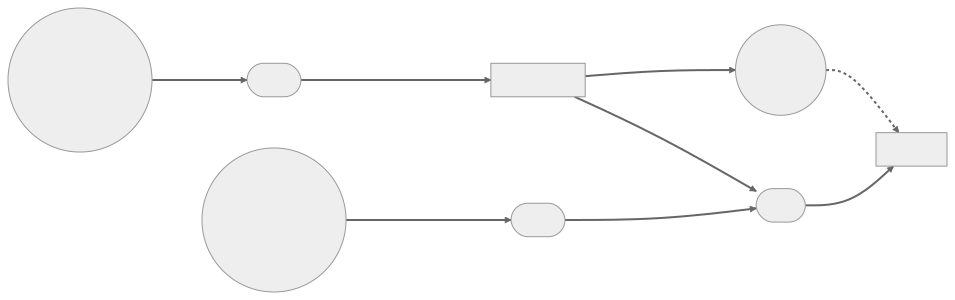
\includegraphics[scale=0.8]{flowcharts/nextflow_dag_v0.2}
	\caption{\Ac{DAG} for Nextflow workflow with added BAM to FastQ file conversion}
	\label{fig:dag_v02}
\end{figure}

An evaluation of the combined workflow is not conducted, as results can be derived from the previous measurements: a genome analysis will take about \SI{1.65}{\hour} longer with BAM to FastQ conversion.

\subsection{Separation of \acs{megSAP} Steps}\label{subsection:seperationofsteps}

To optimize \textit{\ac{megSAP}}'s resource usage, the individual steps \textemdash mapping, variant calling, copy number variant calling, structural variant calling, and database import (see \cref{fig:flowchart_overview}) \textemdash need to be separated. After splitting, each step can be measured on its own by \textit{Nextflow}'s build in HTML execution report (see \autocite{SeqeraLabs2022a}). To accomplish this, the \textit{Nextflow} process \textttx{megSAP} is replaced by five separate processes (\cref{lst:megsapgermlinev03}, line \numrange{27}{100}): \textttx{megSAPma}, \textttx{megSAPvc}, \textttx{megSAPcn}, \textttx{megSAPsv}, and \textttx{megSAPdb}. These processes are nearly identical to the \textttx{megSAP} process in the last iteration, with three changes:
\begin{enumerate}
    \item The variable \textttx{threads} containing the number of threads defined in the \textit{Nextflow} configuration file (e.g., line 39).
    \item The variable \textttx{steps} defining the steps to be run during the execution of \textit{\ac{megSAP}} (e.g., line 40). This variable is the only difference between the newly added process blocks.
    \item The command to call \textit{\ac{megSAP}} has been extracted to a separate script (see \cref{lst:megsapgermlinesh}) in a template folder. The \textttx{template} keyword (e.g., line 41) is used to define a reusable code fragment that can be utilized in multiple places within a workflow. Templates can be parameterized, allowing different values to be passed in each time the template is used, in this case the previous introduced parameters \textttx{containerDirectory} and \textttx{sampleName} accompanied by the new \textttx{threads} and \textttx{steps}. Templates provide a way to factor out common parts of a pipeline and simplify pipeline development, making the code more readable and maintainable. By utilizing this part of \textit{Nextflow}'s \ac{DSL} described in \autocite[Module templates]{SeqeraLabs2022}, this common data processing operation can be shared across all processes calling \textit{\ac{megSAP}}.
\end{enumerate}
Creating multiple process steps instead of implementing a reusable process with a calling parameter to set the \textit{\ac{megSAP}} step is deliberate. Resource allocation in the configuration can only be done by providing the process name or adding a label to a process. Both cannot be changed dynamically. So the goal, setting different resource constraints for each step, cannot be reached without creating multiple process blocks.

The separation shows a direct flow between the consecutive steps in the generated \ac{DAG}, as seen in \cref{fig:dag_v03}.

\begin{figure}[H]
    \centering
	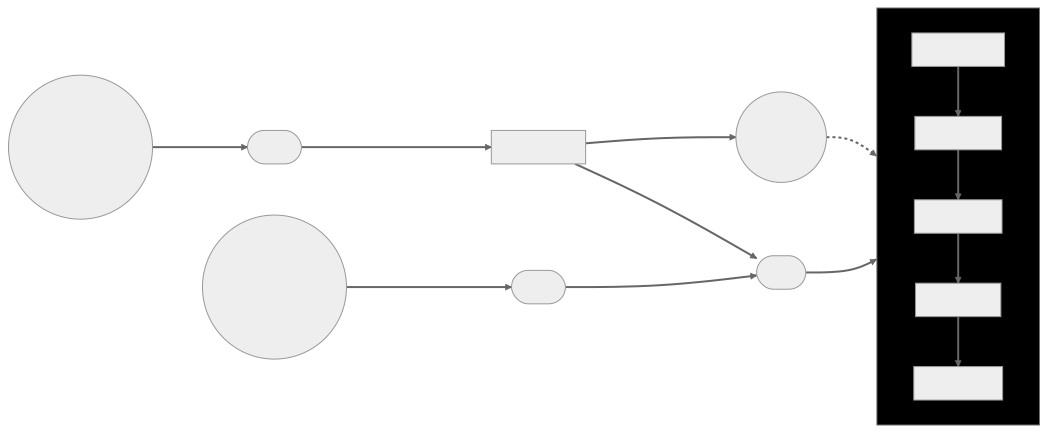
\includegraphics[width=1\textwidth,height=0.9\textheight,keepaspectratio]{flowcharts/nextflow_dag_v0.3}
	\caption{\Ac{DAG} for Nextflow workflow after separation of \acs{megSAP} steps}
	\label{fig:dag_v03}
\end{figure}

The separated workflow ran for approximately \SI{12.9}{\hour} (see \cref{table:megsapgermlinev03benchmark}). This is a little longer than the run without the split. This slight variance is expected, as other process are running on the \ac{HPC} cluster that may have an impact on file read, file write and network performance, and are not controllable. As shown previously in \cref{table:scriptruntimestats}, the standard deviation of pipeline runs in the past was \SI{6.7}{\hour}, well above the observed \SI{1.4}{\hour}. A runtime comparison between all iterations can be found in \cref{subsection:resourceoptimization}, \cref{figure:pipeline_benchmark_runtime}.

The average CPU utilization for each process varies substantially, with the highest utilization being \SI{53.1}{\percent} for the \textttx{megSAPvc} process and the lowest being \SI{1.7}{\percent} for the \textttx{megSAPdb} process as shown in \cref{figure:pipeline_benchmark_CPU_v03}. The peak memory usage also varies significantly among the processes, ranging from \SI{2}{\percent} for the \textttx{megSAPma} process to \SI{81.9}{\percent} for the \textttx{megSAPcn} process, as shown in \cref{figure:pipeline_benchmark_memory_v03}. A representation of the CPU and memory allocation and usage over time can be seen in \cref{figure:pipeline_benchmark_CPU_aoc_v03,figure:pipeline_benchmark_memory_aoc_v03}. Detailed statistics are listed in \cref{table:megsapgermlinev03benchmark}.

\begin{figure}[H]
    \centering
	\includegraphics[width=\linewidth,height=\textheight,keepaspectratio]{pipeline_benchmark_CPU_v03}
	\caption{Average CPU usage of the Nextflow workflow after separation of steps}
	\label{figure:pipeline_benchmark_CPU_v03}
\end{figure}

\begin{figure}[H]
    \centering
	\includegraphics[width=\linewidth,height=\textheight,keepaspectratio]{pipeline_benchmark_memory_v03}
	\caption{Peak memory usage of the Nextflow workflow after separation of steps}
	\label{figure:pipeline_benchmark_memory_v03}
\end{figure}

\begin{figure}[H]
    \centering
	\includegraphics[width=\linewidth,height=\textheight,keepaspectratio]{pipeline_benchmark_CPU_v3_aoc}
	\caption{Average CPU usage of the Nextflow workflow over time after separation of steps}
	\label{figure:pipeline_benchmark_CPU_aoc_v03}
\end{figure}

\begin{figure}[H]
    \centering
	\includegraphics[width=\linewidth,height=\textheight,keepaspectratio]{pipeline_benchmark_memory_v3_aoc}
	\caption{Memory usage of the Nextflow workflow over time after separation of steps}
	\label{figure:pipeline_benchmark_memory_aoc_v03}
\end{figure}

\subsection{Resource Optimization of \acs{megSAP} Steps}\label{subsection:resourceoptimization}

Based on the reported resource usage after the separation of the \textit{\ac{megSAP}} steps, each process is set up with its own resource directives within the \textit{Nextflow} configuration. This is being realized with the \textttx{withName} process selector described in \autocite[Process selectors]{SeqeraLabs2022e}. These allow to set specific parameters only for processes with a particular name. The values themselves are derived from the results shown previously in \cref{figure:pipeline_benchmark_CPU_v03} and \cref{figure:pipeline_benchmark_memory_v03}. This cannot be done as precisely as needed for the CPU requirements, as \textit{Nextflow} measures the weighted average of CPU utilization (see \autocite{SeqeraLabs2022d}). Therefore, a little buffer is added to the CPU allocation. Additionally, the mapping step (\textttx{ma}) has an outstanding characteristic: within this step, \textit{\ac{megSAP}} utilizes two \textit{Illumina DRAGEN} servers (see \autocite{IlluminaInc.2022}) owned by the \ac{DoHG@MHH}. These operate outside the \textit{SLURM} cluster in their own \textit{Sun Grid Engine} environment. Each can process one sample at a time. The external child process is not monitored by \textit{Nextflow}, as \textit{\ac{megSAP}} itself is just idly waiting. This dilutes the CPU related measurements of this step, as it also includes the usage of \textit{SeqPurge} to optimize the data before mapping takes place as described in \autocite{Sturm2016}. That part of the mapping step is best run using 15 threads (see \cref{appendix:correspondecemarc}) resulting in this being set as a configuration parameter. Each process step is also configured with a small buffer of \SI{10}{\percent} (and rounded up to the next even number) to factor in some fluctuation. 

The resulting configuration values are shown in \cref{table:resourceoptimization} and can be seen in the updated configuration in \cref{lst:megsapnextflowconfigv04}.

With this configuration, the pipeline ran for \SI{13.6}{\hour}. See \cref{figure:pipeline_benchmark_runtime} for a comparison between the runtime of all pipeline configurations.

\begin{table}[H]
\centering
\caption{Configured resource allocation after optimization}
\label{table:resourceoptimization}
    \begin{tabularx}{\textwidth}{lYYYYY}
        \toprule
        process & megSAPma & megSAPvc & megSAPcn & megSAPsv & megSAPdb \\ 
        \midrule
        allocated CPUs & \num{15} & \num{8} & \num{2} & \num{2} & \num{2} \\ 
        allocated memory & \SI{2}{\giga\byte} & \SI{20}{\giga\byte} & \SI{48}{\giga\byte} & \SI{2}{\giga\byte} & \SI{2}{\giga\byte} \\
        \bottomrule
    \end{tabularx}
\end{table}

\begin{figure}[H]
    \centering
	\includegraphics[width=\linewidth,height=\textheight,keepaspectratio]{pipeline_benchmark_runtime_v04}
	\caption{Comparison of pipeline runtime over all iterations}
	\label{figure:pipeline_benchmark_runtime}
\end{figure}

The CPU usage of the \textttx{megSAPvc} and \textttx{megSAPcn} steps is decreased, although they still do not use all allocated cores efficiently as shown in \cref{figure:pipeline_benchmark_CPU_v04}. This applies especially to the \textttx{megSAPma} step, but was expected, as described before. Memory usage is reduced in the \textttx{megSAPvc} and \textttx{megSAPcn} steps as well, with the latter not even using half its provided memory resources, as shown in \cref{figure:pipeline_benchmark_memory_v04}. A representation of the CPU and memory allocation and usage of the optimized workflow over time can be seen in \cref{figure:pipeline_benchmark_CPU_aoc_v04,figure:pipeline_benchmark_memory_aoc_v04}. Detailed statistics are listed in \cref{table:megsapgermlinev04benchmark}.

\begin{figure}[H]
    \centering
	\includegraphics[width=\linewidth,height=\textheight,keepaspectratio]{pipeline_benchmark_CPU_v04}
	\caption{Average CPU usage of the Nextflow workflow after optimization}
	\label{figure:pipeline_benchmark_CPU_v04}
\end{figure}

\begin{figure}[H]
    \centering
	\includegraphics[width=\linewidth,height=\textheight,keepaspectratio]{pipeline_benchmark_memory_v04}
	\caption{Peak memory usage of the Nextflow workflow after optimization}
	\label{figure:pipeline_benchmark_memory_v04}
\end{figure}

\begin{figure}[H]
    \centering
	\includegraphics[width=\linewidth,height=\textheight,keepaspectratio]{pipeline_benchmark_CPU_v4_aoc}
	\caption{Average CPU usage of the Nextflow workflow after optimization over time}
	\label{figure:pipeline_benchmark_CPU_aoc_v04}
\end{figure}

\begin{figure}[H]
    \centering
	\includegraphics[width=\linewidth,height=\textheight,keepaspectratio]{pipeline_benchmark_memory_v4_aoc}
	\caption{Memory usage of the Nextflow workflow after optimization over time}
	\label{figure:pipeline_benchmark_memory_aoc_v04}
\end{figure}

\subsection{Resilience and Monitoring}\label{subsection:resilienceandmonitoring}

To make the pipeline less prone to errors, two of \textit{Nextflow}s directives for error handling are introduced to the process configuration (see \cref{appendix:megsapgermlinev1}, \cref{lst:megsapnextflowconfigv1}):
\begin{description}
    \item[\textttx{maxRetries}] This option sets the maximum number of times a task will be re-executed in case of failure (see \autocite[Directives/maxRetries]{Seqeralabs2022f}. This is set to \textttx{2} (line \num{12}).
    \item[\textttx{errorStrategy}] This directive provides the capability to specify how an error should be handled by the process (see \autocite[Directives/errorStrategy]{Seqeralabs2022f}. By default, if an error status is returned by the executed script, the process immediately stops, leading to termination of the entire pipeline. This \textttx{errorStrategy} is called \textttx{terminate}. Other options are:
    \begin{description}[leftmargin=*,widest=ignore]
        \item[\textttx{finish}] Activates a controlled shutdown of the pipeline in response to an error event, while allowing the execution of any submitted tasks to complete.
        \item[\textttx{ignore}] Ignores any execution errors during the process.
        \item[\textttx{retry}] Restarts a process that returns an error condition.
    \end{description}
    To retry a process step after an error, the \textttx{retry} option is chosen. This option falls back to the \textttx{terminate} option if the maximum defined number of retries is reached. If multiple samples are analyzed in one execution of the \textit{Nextflow} workflow, this is not desired, as other samples might process without any errors. Thus, a dynamic approach of setting the \textttx{errorStrategy} is employed, setting the option to \textttx{ignore} in the event of a failed second execution attempt (line \num{13}).
\end{description}

Connecting \textit{Nextflow} to an email server allows for automatic notifications for pipeline completion, whether successful or with errors (see \autocite[Scope mail]{SeqeraLabs2022e}). This is set up in line \numrange{63}{67}.

An evaluation of these changes is not needed, as those neither affect resource consumption nor runtime.
\cleardoublepage
\section{Cost Estimation of Potential Cloud Usage}\label{sec:awscostestimation}

Utilization of cloud computing for the processing of the amount of data to be reanalyzed is a promising approach and a possible solution to the \ac{DoHG@MHH}s problems as outlined in \cref{subsection:goals}. Among cloud providers, \ac{AWS} offers specialized \textit{F1} instances through their \textit{\ac{EC2}} service with \ac{FPGA} support and pre-installed, official \textit{DRAGEN} software. Thus, \ac{AWS} was chosen for this approach.

Costs for cloud computing should be calculated in advance to ensure that the \ac{DoHG@MHH} fully understands the expenses involved and can make an informed decision about whether the benefits of using cloud computing are worth the costs. This includes considering the cost of any additional services or solutions that may be required to address any limitations or challenges posed by cloud computing, such as limited bandwidth.

By using the benchmarking results given by the last iteration of the \textit{Nextflow} implementation, a precise selection of the compute instance is possible regarding the required resource needs of each processing step.

\Ac{AWS} provides a price calculator tool (see \autocite{AmazonWebServices2023}) designed to estimate the cost of using \ac{AWS} services. The calculator considers various factors such as the types of instances used, the number of instances, storage requirements, and data transfer costs to generate a comprehensive estimate of the total cost of using \ac{AWS} services. The tool provides a detailed breakdown of costs by service, region, and usage.

The price calculation for one sample is done with the following assumptions:
\begin{itemize}
    \item A sample takes up \SI{100}{\giga\byte} of space (an approximation, \textit{NA12878} takes up \SI{107}{\giga\byte} for example). This consists of two parts: the uploaded data to be analyzed (either in BAM or FastQ file format), and the analyzation results produced by the pipeline (including the BAM file mapped to \textit{GRCh38}). Both consume an equal size of space.
    \item The lowest possible \textit{\ac{EC2}} \textit{Intel} architecture-based instance configuration fitting to the results obtained in \cref{subsection:resourceoptimization} is used.
    \item The exact usage time measured in \cref{subsection:resourceoptimization} is used as well.
    \item Calculations are done for \textit{\ac{AWS}}' Frankfurt region because of legal and performance reasons.
    \item The step \textttx{megSAPdb} is left out. This has to be done locally at the \ac{DoHG@MHH} to use the data in its database. Its resource consumption is negligible, as shown previously.
    \item Data storage and transfer is calculated based on one sample. Pricing for more storage and data transfer may be cheaper in bulk.
\end{itemize}

Price calculations for the use of the specialized \textit{DRAGEN} equipped \textit{F1} instances of \textit{\ac{EC2}} are not possible with the price calculator tool, but can be done via the product page (\autocite{AmazonWebServices2023a}). Analyzing \textit{\ac{megSAP}}'s log files show that the \textit{DRAGEN} part of the mapping step takes approximately one hour. Using the f1.2xlarge instance type, this will amount to \SI{12.08}{\$}. The calculated cost for all other services, including an overview of the selected \textit{EC2} instance types, is detailed in \cref{table:awscostandtypes} and amounts to \SI{14.25}{\$}, bringing the total cost for one sample to \SI{26.33}{\$} (if retained on the \textit{S3} storage for a maximum of one month).

Given the number of samples calculated in \cref{subsection:problem}, the total cost to reanalyze in the cloud would sum up to $\SI{1544}{\text{samples}}\times\SI{26.33}{\$}=\SI{40653.52}{\$}$.

To handle the upload of all data currently archived at the \ac{DoHG@MHH}, an \textit{\ac{AWS} Snowball} edge storage device may be used instead of straining the relatively slow upload capacity provided. The approximately \SI{77.2}{\tera\byte} (see \cref{subsection:problem}) of data would fit on one device. Assuming the data transfer at the \ac{DoHG@MHH} can be completed in \SI{10}{\day}, which is feasible, the cost would be \SI{300}{\$} (see \autocite{AmazonWebServices2023b}), with an additional \SI{30}{\$} for each additional day.

This removes half of the data transfer costs (only the upload, not the download of the analyzed data), bringing the total down to $\SI{40653.52}{\$}-\left(\frac{\SI{4.50}{\$}}{2}\times1544\right)+\SI{300}{\$}=\SI{37479.52}{\$}$.

\begin{table}[H]
    \centering
    \caption{Results of \ac{AWS} price calculator tool and selected instance types}{Details can be found in \cref{appendix:awspricecalculationoptimized}.\\\smallskip}
    \label{table:awscostandtypes}
    \begin{tabularx}{\textwidth}{lXYYY}
        \toprule
        Description/Process & EC2 instance type & CPUs & Memory in GB & Cost in \unit{\$} \\
        \midrule
        Storage & & & & 2.45 \\ 
        Data Transfer & & & & 4.50 \\
        bam2fastq & t3.large & 2 & 8 & 0.16 \\
        megSAPma & c6i.4xlarge & 16 & 32 & 2.08 \\ 
        megSAPvc & t3.2xlarge & 8 & 32 & 1.15 \\ 
        megSAPcn & r5.2xlarge & 8 & 64 & 3.88 \\ 
        megSAPsv & t3.small & 2 & 2 & 0.04 \\
        \bottomrule
    \end{tabularx}
\end{table}

\cleardoublepage
\section{Discussion}\label{sec:discussion}

The separation of pipeline steps and their individual resource allocation allows for a more efficient usage of the \ac{HPC} cluster. Previously unnecessarily reserved threads and memory can now be used to process more samples in parallel. More resources can be utilized in parallel, as shown in \cref{subsection:resourceoptimization} and visualized side-by-side in \cref{figure:pipeline_benchmark_CPU_compared} and \cref{figure:pipeline_benchmark_memory_compared}.

\begin{figure}[H]
    \centering
	\includegraphics[width=\linewidth,height=\textheight,keepaspectratio]{pipeline_benchmark_CPU_compared}
	\caption{Average CPU usage of the Nextflow workflows compared}
	\label{figure:pipeline_benchmark_CPU_compared}
\end{figure}

\begin{figure}[H]
    \centering
	\includegraphics[width=\linewidth,height=\textheight,keepaspectratio]{pipeline_benchmark_memory_compared}
	\caption{Peak memory usage of the Nextflow workflows compared}
	\label{figure:pipeline_benchmark_memory_compared}
\end{figure}

To quantify the gains, the measuring unit \textit{CPU hours} respectively \textit{memory hours} is calculated for the reserved resources. As seen in \cref{equation:initialcpu,equation:initialmemory}, this resolves to \SI{138.0}{CPU~\hour} and \SI{575}{\giga\byte~\hour} for the initial workflow described in \cref{subsection:initialworkflow}.
\begin{equation}\label{equation:initialcpu}
    \begin{aligned}
        \SI{12}{CPU}\times\SI{11.5}{\hour} &= \SI{138.0}{CPU~\hour}
    \end{aligned}
\end{equation}
\begin{equation}\label{equation:initialmemory}
    \begin{aligned}
        \SI{50}{\giga\byte}\times\SI{11.5}{\hour} &= \SI{575}{\giga\byte~\hour}
    \end{aligned}
\end{equation}

After optimization, the result is \SI{79.563}{CPU~\hour} for reserved CPU resources and \SI{374.501}{\giga\byte~\hour} for memory as calculated in \cref{equation:optimizedcpu,equation:optimizedmemory} 
\begin{equation}\label{equation:optimizedcpu}
    \begin{aligned}
        \text{megSAPma: }\SI{15}{CPU}\times\SI{2.683}{\hour} &= \SI{40.245}{CPU~\hour}\\
        \text{megSAPvc: }\SI{8}{CPU}\times\SI{2.938}{\hour} &= \SI{23.504}{CPU~\hour}\\
        \text{megSAPcn: }\SI{2}{CPU}\times\SI{6.383}{\hour} &= \SI{12.766}{CPU~\hour}\\
        \text{megSAPsv: }\SI{2}{CPU}\times\SI{1.467}{\hour} &= \SI{2.934}{CPU~\hour}\\
        \text{megSAPdb: }\SI{2}{CPU}\times\SI{0.057}{\hour} &= \SI{0.114}{CPU~\hour}\\
        \hline
        \text{Optimized workflow } &= \SI{79.563}{CPU~\hour}
    \end{aligned}
\end{equation}
\begin{equation}\label{equation:optimizedmemory}
    \begin{aligned}
        \text{megSAPma: }\SI{2}{\giga\byte}\times\SI{2.683}{\hour} &= \SI{5.366}{\giga\byte~\hour}\\
        \text{megSAPvc: }\SI{20}{\giga\byte}\times\SI{2.938}{\hour} &= \SI{59.76}{\giga\byte~\hour}\\
        \text{megSAPcn: }\SI{48}{\giga\byte}\times\SI{6.383}{\hour} &= \SI{306.384}{\giga\byte~\hour}\\
        \text{megSAPsv: }\SI{2}{\giga\byte}\times\SI{1.467}{\hour} &= \SI{2.934}{\giga\byte~\hour}\\
        \text{megSAPdb: }\SI{1}{\giga\byte}\times\SI{0.057}{\hour} &= \SI{0.057}{\giga\byte~\hour}\\
        \hline
        \text{Optimized workflow } &= \SI{374.501}{\giga\byte~\hour}
    \end{aligned}
\end{equation}
This means that CPU resources are used \SI{42.35}{\percent} more efficient than before and memory is used \SI{34.87}{\percent} more economically after the optimizations as also shown in \cref{figure:pipeline_benchmark_efficiency}. 

A comparison of initial and optimized CPU and memory allocation over time is shown in \cref{figure:pipeline_cpu_compared_aoc,figure:pipeline_memory_compared_aoc}

\begin{figure}[H]
    \centering
	\includegraphics[width=\linewidth,height=\textheight,keepaspectratio]{pipeline_benchmark_efficiency}
	\caption{Efficiency after pipeline optimization}{Resource consumption of the megSAPdb process is too low to be rendered.}
	\label{figure:pipeline_benchmark_efficiency}
\end{figure}

\begin{figure}[H]
    \centering
	\includegraphics[width=\linewidth,height=\textheight,keepaspectratio]{pipeline_benchmark_CPU_compared_aoc}
	\caption{CPU allocation of initial and optimized workflows over time}
	\label{figure:pipeline_cpu_compared_aoc}
\end{figure}

\begin{figure}[H]
    \centering
	\includegraphics[width=\linewidth,height=\textheight,keepaspectratio]{pipeline_benchmark_memory_compared_aoc}
	\caption{Memory allocation of initial and optimized workflows over time}
	\label{figure:pipeline_memory_compared_aoc}
\end{figure}

This can also be transferred to the estimated cost of using \textit{\ac{AWS}} to compute the pipeline in the cloud. With the optimized pipeline, this amounts to \SI{26.33}{\$} as shown in \cref{sec:awscostestimation}. Using a m5.4xlarge instance type to run the pipeline in its previous state (see \cref{subsection:initialworkflow}) for \SI{11.5}{\hour} would raise this to \SI{29.77}{\$} (see \cref{appendix:awspricecalculationunoptimized} for details), saving \SI{11.56}{\percent}. This amount is lower than the realizable retrenchments for the \ac{HPC} cluster, as \textit{\ac{AWS}} instance types do not exactly match to the required resources and the overhead produces more cost than necessary.

These resource adjustments should be monitored and improved upon in the future. Slight changes might show improvements on execution time or allow for less resources to be allocated to some steps. A first example might be the \textttx{megSAPcn} step. Its memory consumption seems to be affected by the number of threads, as it dropped more than half after reducing the number of available CPUs.

Two different approaches can be taken to optimize the resource usage: 
\begin{enumerate}
    \item Using resources to process a sample as fast as possible. This may be needed to answer a particular time critical diagnostic question.
    \item Using resources to process multiple samples simultaneously as efficient as possible. Routine diagnostic profits from an average optimal processing time calculated over multiple samples. 
\end{enumerate}
As resource usage and runtime do not correlate linearly, but probably follow more of a sigmoid curve, these two approaches differ. For this thesis, the latter approach has been taken, as its goal is to process numerous samples retroactively. But the \ac{DoHG@MHH} sometimes has different needs regarding the speed of diagnostics, e.g., for the \textit{Baby Lion} study (see \autocite{MedizinischeHochschuleHannover2022}), which employs rapid whole-genome sequencing as described by \citeauthor{Saunders2012} \autocite{Saunders2012}, the pipeline should run as fast as possible. Handling both approaches may be put into practice for the \textit{Nextflow} pipeline by using different configuration profiles (see \autocite[Config profiles]{SeqeraLabs2022e}) for different needs.

Since the CPU utilization is only calculated as a weighted average, thread allocation is an explorative task. Additionally, \textit{\ac{megSAP}} combines too many tools into one step to make informed decisions on thread usage. This is particularly visible in the mapping step, as outlined in \cref{subsection:seperationofsteps}: The resource-intensive task \textit{SeqPurge} is combined with the, at least from a cluster perspective, idling task that waits for the \textit{DRAGEN} mapping to be done. To facilitate more optimization in the future, \textit{\ac{megSAP}} has to be separated into more individual steps. At best, each tool has its own process in \textit{Nextflow} in the future \textemdash this would render all the current \textit{PHP} scripts of \textit{\ac{megSAP}} obsolete and move all logic to \textit{Nextflow} - a vision worth considering.

Otherwise, the memory utilization is measured by peak usage and the optimization for each step, as presented in \cref{subsection:resourceoptimization}, can approach this optimum. These optimizations would also benefit from a fragmentation of the \textit{\ac{megSAP}} steps, as changes could be more precise and not only accommodate for the extremum usage of a whole pipeline step, but for each tool used \textemdash in the same manner as the CPU usage optimizations.

One pertinent measurement was not included for this thesis: disk utilization. The \ac{HPC} cluster does not have tiered storage. All data resides on the same network attached storage. Therefore, no actions could have been derived by any findings. But as the operations performed by the pipeline are using large files to begin with, it might be a promising endeavor to employ faster scratch devices during the pipeline run.

The implementation of \textit{Nextflow} also introduces a remedy for previous problems:
\begin{description}
    \item[Resilience] By leveraging \textit{Nextflow}'s built-in \textttx{maxRetries} directive (see \cref{subsection:resilienceandmonitoring}) it is possible to cure not reproducible pipeline errors. By simply restarting the relevant step with more resources, these errors can be automatically fixed.
    
    Nevertheless, it might be expedient to check for certain error-codes to react accordingly. For example, an out-of-memory error could be fixed systematically instead of just blindly trying the failed step again with more resources.
    
    \item[Reporting] The email reporting features of \textit{Nextflow} are a first step towards better monitoring of the pipeline. This also applies to the detailed reports generated by each workflow run.
\end{description}

The created \textit{Nextflow} workflow is hosted on the \ac{MHH}'s internal \textit{GitLab} severs. Using \textit{Git} as a version control system allows for tracking changes made to the workflow over time, so it can easily be reverted to previous versions if needed. Hosting the workflows in \textit{GitLab} also provides a backup and helps to ensure that the workflow is not lost in case of any data loss. \textit{GitLab} also makes it easier to share the workflow and to reuse it in different projects.

Two issues outlined in \cref{subsection:problem} were not fixed by the initial introduction of \textit{Nextflow}: the workflow still has to be triggered by a shell command and no accessible monitoring is possible during the pipeline run. Both of these impediments might be fixable by harnessing the features offered by \textit{Nextflow Tower} (see \autocite{SeqeraLabs2022g}). It promises enhanced monitoring, logging, and observability for workflows and streamlined deployment of pipelines by providing a easy to use web-based interface. Incorporating \textit{Nextflow Tower} into the newly built \textit{Nextflow} workflow will be the next project at the \ac{DoHG@MHH}.

\cleardoublepage
\section{Conclusion}\label{sec:conclusion}

In conclusion, this bachelor thesis provides a comprehensive insight on the significance of implementing a \acl{SWfMS} to support the transition to a newer reference genome, in this case \textit{GRCh38}. By leveraging the included resource usage reports of the chosen solution \textit{Nextflow}, it is possible to improve the efficiency of the genetic analysis pipeline greatly, with a reduction in resource usage by over a third. 

The adoption of \textit{Nextflow} represents the beginning of a journey for the \ac{DoHG@MHH} to use their genetic analyzation pipeline more professional. This work lays the foundation for further advancements, such as the separation of \textit{\ac{megSAP}} steps and the addition of \textit{Nextflow Tower}. These suggestions, if implemented, would provide the \ac{DoHG@MHH} with even greater benefits in terms of efficiency, accessibility, and usability.

One of the main challenges that the \ac{DoHG@MHH} faces is limited processing capacity, which has been remedied by the implementation of \textit{Nextflow}. In addition, the cost of using cloud infrastructure has also been presented as a possible solution in the future. The use of cloud infrastructure would provide the \ac{DoHG@MHH} with unlimited processing capacity, and therefore, the ability to perform genetic analyses with as much parallelism as needed. Especially for the task at hand, to reanalyze all old samples with a new reference genome without disturbing regular diagnostics, the cost of such an endeavor might be worth it.

The results of this thesis demonstrate that the implementation of a \ac{SWfMS} into the genetic analysis pipeline has many benefits, not only in terms of efficiency and accuracy, but also in terms of future scalability. This transition to \textit{GRCh38} has been made possible due to the use of \textit{Nextflow}, and the results will be transferred to the routine medical diagnostics pipeline, as \textit{Nextflow} will be adopted there. The migration will be seamless, with the current scripts being replaced by a script that starts the new \textit{Nextflow} workflow.

Finally, this thesis provides a clear and concise overview of the implementation of a \ac{SWfMS} to support the transition to a new reference genome. The results demonstrate that the use of \textit{Nextflow} is an effective solution, not only for the \ac{DoHG@MHH}, but also for any laboratory that needs to transition to a new reference genome. The benefits of using a \ac{SWfMS}, such as \textit{Nextflow}, are numerous and include improved efficiency, scalability, and cost savings. This thesis serves as a blueprint for the successful implementation of a \ac{SWfMS} in a genetic analysis pipeline and provides a roadmap for future improvements and advancements.

\cleardoublepage
\printbibliography[heading=bibintoc]

\cleardoublepage
\appendix
\addsec{Appendix}
\renewcommand{\thesubsection}{\Roman{subsection}}
\subsection{Sum of Processed Samples}

The sum of processed samples has been generated by a query to the database (see \autoref{lst:sqlprocessedsamples}) of the \ac{DoHG@MHH}'s \ac{LIMS}.

\begin{table}[H]
\centering
\caption{Sum of processed samples at the \acs{DoHG@MHH} per year}
\label{tab:sum_of_samples}
\begin{tabular}{lr}
\toprule
Year & Sum of processed samples \\
\midrule
2016 & 37 \\
2017 & 292 \\
2018 & 466 \\
2019 & 661 \\
2020 & 1460 \\
2021 & 1794 \\
\bottomrule
\end{tabular}
\end{table}

\lstinputlisting[language=sql, caption={SQL for sum of processed samples},captionpos=t, label=lst:sqlprocessedsamples]{listings/sum_of_samples.sql}

\clearpage
\subsection{Extrapolation of Whole-Genome Samples Analyzed Until Project Deadline}\label{appendix:extrapolation}
Data for the first four months of the year 2022 has been generated by a query to the database (\autoref{lst:wholegenome2022extrapolationsql}) and extrapolated by calculating the least squares fit (see \autocite{NumPyDevelopers2022}) with a python script (\autoref{lst:wholegenome2022extrapolationpy}).

\lstinputlisting[language=sql, caption={SQL query to gather data for extrapolation}, captionpos=t, label=lst:wholegenome2022extrapolationsql]{listings/whole_genome_2022_extrapolation.sql}

\lstinputlisting[language=python, caption={Python code to extrapolate the sum of whole-genome sequencing runs until the project's deadline}, captionpos=t, label=lst:wholegenome2022extrapolationpy]{listings/whole_genome_2022_extrapolation.py}


\clearpage
\subsection{Example Script of Pipeline Invocation with Bash}\label{appendix:bashscript}
\lstinputlisting[language=bash, caption={bash script to trigger the \acs{megSAP} pipeline}, captionpos=t, label=lst:pipelinescriptold]{listings/make_analyze_12c_slurm_IDTPanelV2_GRCh38_dragen.sh}

\clearpage
\subsection{Initial Nextflow Workflow}\label{appendix:megsapgermlinev01}
\lstinputlisting[caption={megsap\_germline.nf (Initial Version)}, captionpos=t, label=lst:megsapgermlinev01]{listings/megsap_germline_v0.1.nf}
\lstinputlisting[caption={nextflow.config (Initial Version)}, captionpos=t, label=lst:megsapnextflowconfigv01]{listings/nextflow_v0.1.config}

\begin{table}[H]
\centering
\caption{Reported resource usage for initial workflow}
\label{table:megsapgermlinev01benchmark}
    \begin{tabular}{lr}
        \toprule
        process & megSAP \\ 
        \toprule
        allocated cpus & \num{12} \\ 
        \%cpu & \num{294.2} \\ 
        allocated memory & \SI{50}{\giga\byte} \\ 
        peak\_vmem & \SI{42.752}{\giga\byte} \\ 
        duration & \SI{11}{\hour} \SI{36}{\minute} \\ 
        read\_bytes & \SI{421.380}{\giga\byte} \\ 
        write\_bytes & \SI{303.939}{\giga\byte} \\ 
        \bottomrule
\end{tabular}
\end{table}

\clearpage
\subsection{Detailed Data of BAM to FastQ Conversion Benchmarks}
\begin{table}[H]
\centering
\caption[Statistics of samples used for benchmarking BAM to FastQ conversion using the command samtools flagstat]{Statistics of samples used for benchmarking BAM to FastQ conversion using the command \textttx{samtools flagstat} (see \autocite{GenomeResearchLimited2022})}
\label{table:bam2fastq_benchmark_sample_stats}
\small
\begin{tabularx}{\textwidth}{Xyy}
\toprule
& whole exome sample reads & whole genome sample reads \\ \midrule
in total (QC-passed reads + QC-failed reads) & \num{94905155} & \num{945531162} \\
primary & \num{93901428} & \num{934455908} \\
secondary & \num{0} & \num{0} \\
supplementary & \num{1003727} & \num{11075254} \\
duplicates & \num{3912559} & \num{88969100} \\
primary duplicates & \num{3866188} & \num{88113730} \\
mapped & \num{94564593} & \num{943533900} \\
primary mapped & \num{93560866} & \num{932458646} \\
paired in sequencing & \num{93901428} & \num{934455908} \\
read1 & \num{46950714} & \num{467227954} \\
read2 & \num{46950714} & \num{467227954} \\
properly paired & \num{89632844} & \num{873201928} \\
with itself and mate mapped & \num{93324280} & \num{931711492} \\
singletons & \num{236586} & \num{747154} \\
with mate mapped to a different chr & \num{3227688} & \num{23593106} \\
with mate mapped to a different chr (mapQ\textgreater{}=5) & \num{2383985} & \num{17533528} \\
\bottomrule
\end{tabularx}
\end{table}

\begin{table}[H]
\centering
\caption{Duration of BAM to FastQ conversion of whole exome data by tool in minutes}
\label{table:bam2fastqduration}
\small
\begin{tabularx}{\textwidth}{lYYYYYYY}
\toprule
type & mean & std & min & 25\% & 50\% & 75\% & max \\
\midrule
biobambam2 & 34.81 & 0.36 & 34.40 & 34.49 & 34.73 & 35.17 & 35.24 \\
ngs-bits & 12.09 & 0.09 & 11.99 & 12.03 & 12.07 & 12.11 & 12.31 \\
Picard & 17.04 & 0.26 & 16.79 & 16.91 & 16.94 & 17.04 & 17.66 \\
SAMtools multithread & 18.78 & 0.16 & 18.56 & 18.63 & 18.87 & 18.91 & 18.98 \\
SAMtools singlethread & 59.69 & 0.64 & 58.91 & 59.03 & 59.93 & 60.09 & 60.59 \\
\bottomrule
\end{tabularx}
\end{table}

\begin{table}[H]
\centering
\caption{Memory usage of BAM to FastQ conversion of whole exome data by tool}
\label{table:bam2fastqmemory}
\small
\begin{tabularx}{\textwidth}{lYYYYYYY}
\toprule
tool & mean & std & min & 25\% & 50\% & 75\% & max \\
\midrule
biobambam2 & \SI{143}{\mega\byte} & \SI{111}{\kilo\byte} & \SI{143}{\mega\byte} & \SI{143}{\mega\byte} & \SI{143}{\mega\byte} & \SI{143}{\mega\byte} & \SI{143}{\mega\byte} \\
ngs-bits & \SI{768}{\mega\byte} & \SI{1}{\mega\byte} & \SI{766}{\mega\byte} & \SI{766}{\mega\byte} & \SI{768}{\mega\byte} & \SI{769}{\mega\byte} & \SI{769}{\mega\byte} \\
Picard & \SI{2}{\giga\byte} & \SI{23}{\mega\byte} & \SI{2}{\giga\byte} & \SI{2}{\giga\byte} & \SI{2}{\giga\byte} & \SI{2}{\giga\byte} & \SI{2}{\giga\byte} \\
SAMtools multithread & \SI{2}{\giga\byte} & \SI{1}{\mega\byte} & \SI{2}{\giga\byte} & \SI{2}{\giga\byte} & \SI{2}{\giga\byte} & \SI{2}{\giga\byte} & \SI{2}{\giga\byte} \\
SAMtools singlethread & \SI{870}{\mega\byte} & \SI{602}{\kilo\byte} & \SI{870}{\mega\byte} & \SI{870}{\mega\byte} & \SI{870}{\mega\byte} & \SI{870}{\mega\byte} & \SI{872}{\mega\byte} \\
\bottomrule
\end{tabularx}
\end{table}

\begin{table}[H]
\centering
\caption{Amount of data read by BAM to FastQ conversion of whole exome data by tool}
\label{table:bam2fastqioread}
\small
\begin{tabularx}{\textwidth}{lYYYYYYY}
\toprule
tool & mean & std & min & 25\% & 50\% & 75\% & max \\
\midrule
biobambam2 & \SI{9}{\giga\byte} & \SI{24}{\mega\byte} & \SI{9}{\giga\byte} & \SI{9}{\giga\byte} & \SI{9}{\giga\byte} & \SI{9}{\giga\byte} & \SI{9}{\giga\byte} \\
ngs-bits & \SI{8}{\giga\byte} & \SI{42}{\kilo\byte} & \SI{8}{\giga\byte} & \SI{8}{\giga\byte} & \SI{8}{\giga\byte} & \SI{8}{\giga\byte} & \SI{8}{\giga\byte} \\
Picard & \SI{37}{\giga\byte} & \SI{248}{\kilo\byte} & \SI{37}{\giga\byte} & \SI{37}{\giga\byte} & \SI{37}{\giga\byte} & \SI{37}{\giga\byte} & \SI{37}{\giga\byte} \\
SAMtools multithread & \SI{29}{\giga\byte} & \SI{43}{\kilo\byte} & \SI{29}{\giga\byte} & \SI{29}{\giga\byte} & \SI{29}{\giga\byte} & \SI{29}{\giga\byte} & \SI{29}{\giga\byte} \\
SAMtools singlethread & \SI{29}{\giga\byte} & \SI{50}{\kilo\byte} & \SI{29}{\giga\byte} & \SI{29}{\giga\byte} & \SI{29}{\giga\byte} & \SI{29}{\giga\byte} & \SI{29}{\giga\byte} \\
\bottomrule
\end{tabularx}
\end{table}

\begin{table}[H]
\centering
\caption{Amount of data written by BAM to FastQ conversion of whole exome data by tool}
\label{table:bam2fastqiowrite}
\small
\begin{tabularx}{\textwidth}{lYYYYYYY}
\toprule
tool & mean & std & min & 25\% & 50\% & 75\% & max \\
\midrule
biobambam2 & \SI{6}{\giga\byte} & \SI{0}{\byte} & \SI{6}{\giga\byte} & \SI{6}{\giga\byte} & \SI{6}{\giga\byte} & \SI{6}{\giga\byte} & \SI{6}{\giga\byte} \\
ngs-bits & \SI{7}{\giga\byte} & \SI{0}{\byte} & \SI{7}{\giga\byte} & \SI{7}{\giga\byte} & \SI{7}{\giga\byte} & \SI{7}{\giga\byte} & \SI{7}{\giga\byte} \\
Picard & \SI{34}{\giga\byte} & \SI{265}{\kilo\byte} & \SI{34}{\giga\byte} & \SI{34}{\giga\byte} & \SI{34}{\giga\byte} & \SI{34}{\giga\byte} & \SI{34}{\giga\byte} \\
SAMtools multithread & \SI{30}{\giga\byte} & \SI{6}{\kilo\byte} & \SI{30}{\giga\byte} & \SI{30}{\giga\byte} & \SI{30}{\giga\byte} & \SI{30}{\giga\byte} & \SI{30}{\giga\byte} \\
SAMtools singlethread & \SI{30}{\giga\byte} & \SI{0}{\byte} & \SI{30}{\giga\byte} & \SI{30}{\giga\byte} & \SI{30}{\giga\byte} & \SI{30}{\giga\byte} & \SI{30}{\giga\byte} \\
\bottomrule
\end{tabularx}
\end{table}

\begin{table}[H]
\centering
\caption{Duration of BAM to FastQ conversion of whole genome data by tool in hours}
\label{table:bam2fastqdurationgenome}
\small
\begin{tabular}{lr}
\toprule
type & duration in h \\
\midrule
biobambam2 & 3.73 \\
ngs-bits & 1.65 \\
Picard & 2.93 \\
SAMtools multithread & 2.41 \\
SAMtools singlethread & 7.85 \\
\bottomrule
\end{tabular}
\end{table}

\clearpage
\subsection{Nextflow Workflow with added BAM to FastQ File Conversion}\label{appendix:megsapgermlinev02}
\lstinputlisting[caption={megsap\_germline.nf (with added BAM to FastQ File Conversion)}, captionpos=t, label=lst:megsapgermlinev02]{listings/megsap_germline_v0.2.nf}
\lstinputlisting[caption={nextflow.config (with added BAM to FastQ File Conversion)}, captionpos=t, label=lst:megsapnextflowconfigv02]{listings/nextflow_v0.2.config}

\clearpage
\subsection{Nextflow Workflow With Separated Process Steps}\label{appendix:megsapgermlinev03}

\lstinputlisting[caption={megsap\_germline.nf (with separated process steps)}, captionpos=t, label=lst:megsapgermlinev03]{listings/megsap_germline_v0.3.nf}
\lstinputlisting[language=bash, caption={megsap\_germline.sh}, captionpos=t, label=lst:megsapgermlinesh]{listings/megsap_germline.sh}

\begin{table}[H]
\centering
\caption{Reported resource usage for workflow with separated process steps}
\label{table:megsapgermlinev03benchmark}
    \begin{tabularx}{\textwidth}{nrrrrr}
        \toprule
        process & megSAPma & megSAPvc & megSAPcn & megSAPsv & megSAPdb \\ 
        \midrule
        allocated cpus & \num{12} & \num{12} & \num{12} & \num{12} & \num{12} \\ 
        \%cpu & \num{344.8} & \num{636.8} & \num{103.0} & \num{188.1} & \num{20.9} \\ 
        allocated memory & \SI{50}{\giga\byte} & \SI{50}{\giga\byte} & \SI{50}{\giga\byte} & \SI{50}{\giga\byte} & \SI{50.000}{\giga\byte} \\ 
        peak\_vmem & \SI{1.313}{\giga\byte} & \SI{17.595}{\giga\byte} & \SI{43.140}{\giga\byte} & \SI{1.319}{\giga\byte} & \SI{456.023}{\mega\byte} \\ 
        duration & \SI{2}{\hour} \SI{54}{\minute} & \SI{2}{\hour} \SI{40}{\minute} & \SI{6}{\hour} \SI{11}{\minute} & \SI{1}{\hour} \SI{3}{\minute} & \SI{3}{\minute} \SI{51}{\second} \\ 
        \bottomrule
    \end{tabularx}
\end{table}

\clearpage
\subsection{Nextflow Workflow With Resource Optimization}\label{appendix:megsapgermlinev04}
\lstinputlisting[caption={nextflow.config (with resource optimization)}, captionpos=t, label=lst:megsapnextflowconfigv04]{listings/nextflow_v0.4.config}

\begin{table}[H]
    \centering
    \caption{Reported resource usage for workflow with resource optimization}
    \label{table:megsapgermlinev04benchmark}
    \begin{tabularx}{\textwidth}{nrrrrr}
    \toprule
        process & megSAPma & megSAPvc & megSAPcn & megSAPsv & megSAPdb \\ 
        \midrule
        allocated cpus & \num{15} & \num{8} & \num{2} & \num{2} & \num{2} \\ 
        \%cpu & \num{316.6} & \num{470.4} & \num{93.6} & \num{181.9} & \num{22.8} \\ 
        allocated memory & \SI{2}{\giga\byte} & \SI{20}{\giga\byte} & \SI{48}{\giga\byte} & \SI{2}{\giga\byte} & \SI{1}{\giga\byte} \\ 
        peak\_vmem & \SI{1.251}{\giga\byte} & \SI{14.999}{\giga\byte} & \SI{18.786}{\giga\byte} & \SI{1.210}{\giga\byte} & \SI{455.805}{\mega\byte} \\ 
        duration & \SI{2}{\hour} \SI{41}{\minute} & \SI{2}{\hour} \SI{59}{\minute} & \SI{6}{\hour} \SI{23}{\minute} & \SI{1}{\hour} \SI{28}{\minute} & \SI{3}{\minute} \SI{26}{\second} \\
        \bottomrule
    \end{tabularx}
\end{table}

\subsection{Correspondence with Dr. Marc Sturm Discussing CPU Usage of SeqPurge}\label{appendix:correspondecemarc}
\begin{figure}[H]
    \centering
	\includegraphics[width=0.9\textwidth,height=0.9\textheight,keepaspectratio,page=1]{correspondence_sturm_seqpurge}
	\caption[Correspondence with Dr. Marc Sturm discussing CPU usage of SeqPurge]{Correspondence with Dr. Marc Sturm discussing CPU usage of \textit{SeqPurge}}
	\label{fig:correspondecemarc}
\end{figure}
\begin{figure}[H]\ContinuedFloat
    \centering
	\includegraphics[width=0.9\textwidth,height=0.9\textheight,keepaspectratio,page=2]{correspondence_sturm_seqpurge}
	\caption{Correspondence with Dr. Marc Sturm discussing CPU usage of SeqPurge (cont.)}
\end{figure}

\clearpage
\subsection{Nextflow Workflow With Resilience and Monitoring}\label{appendix:megsapgermlinev1}
\lstinputlisting[caption={nextflow.config (with resilience and monitoring)}, captionpos=t, label=lst:megsapnextflowconfigv1]{listings/nextflow_v1.0.config}

\clearpage
\subsection{\ac{AWS} Prize Calculation for Optimized Nextflow Workflow}\label{appendix:awspricecalculationoptimized}
\begin{figure}[H]
    \centering
	\includegraphics[width=1\textwidth,height=0.9\textheight,keepaspectratio,page=1]{AWS_Price_Calculation_One_Sample}
	\caption{\ac{AWS} prize calculation for optimized Nextflow workflow}
\end{figure}
\begin{figure}[H]\ContinuedFloat
    \centering
	\includegraphics[width=1\textwidth,height=0.9\textheight,keepaspectratio,page=2]{AWS_Price_Calculation_One_Sample}
	\caption{\ac{AWS} prize calculation for optimized Nextflow workflow (cont.)}
\end{figure}

\clearpage
\subsection{\ac{AWS} Prize Calculation for initial Nextflow Workflow}\label{appendix:awspricecalculationunoptimized}
\begin{figure}[H]
    \centering
	\includegraphics[width=1\textwidth,height=0.9\textheight,keepaspectratio,page=1]{AWS_Price_Calculation_One_Sample_unoptimized}
	\caption{\ac{AWS} prize calculation for initial Nextflow workflow}
\end{figure}
\begin{figure}[H]\ContinuedFloat
    \centering
	\includegraphics[width=1\textwidth,height=0.9\textheight,keepaspectratio,page=2]{AWS_Price_Calculation_One_Sample_unoptimized}
	\caption{\ac{AWS} prize calculation for initial Nextflow workflow (cont.)}
\end{figure}

%\cleardoublepage
%\pagenumbering{gobble}
%\input{ee}

\end{document}